\documentclass[final,5p]{elsarticle}
\usepackage{amsmath,amssymb,amsfonts}
\usepackage{microtype,pifont}
\usepackage{graphicx}
\usepackage[dvipsnames]{xcolor}
\usepackage{pgfplots}
\usepgfplotslibrary{groupplots}
\pgfplotsset{compat=1.18}
\usepackage{booktabs,multirow,tabularx,array,makecell}
\usepackage{algorithm,algorithmicx,algpseudocode}
\usepackage{enumitem, float,placeins}
\usepackage{caption}
\usepackage[colorlinks,bookmarksopen,bookmarksnumbered,citecolor=blue, colorlinks=true,linkcolor=blue,urlcolor=blue,breaklinks=true]{hyperref}
\usepackage{xurl}
\usepackage{orcidlink}
\usepackage{balance}
% \setlength{\emergencystretch}{3em}
% \Urlmuskip=0mu plus 1mu

% =========================
% Commands and styles
% =========================
\newcommand{\cmark}{\textcolor{ForestGreen}{\ding{51}}}
\newcommand{\xmark}{\textcolor{BrickRed}{\ding{55}}}

\newcolumntype{R}[1]{>{\raggedleft\arraybackslash}m{#1}}
\newcolumntype{L}[1]{>{\raggedright\arraybackslash}m{#1}}
\newcolumntype{C}[1]{>{\centering\arraybackslash}m{#1}}

\renewcommand{\algorithmicrequire}{\textbf{Input:}}
\renewcommand{\algorithmicensure}{\textbf{Output:}}
\algrenewcommand\algorithmiccomment[1]{\hfill{\footnotesize$\triangleright$ #1}}

\makeatletter
\newcommand{\algorithmautorefname}{Algorithm}
\renewcommand{\figureautorefname}{Figure}
\renewcommand{\tableautorefname}{Table}
\renewcommand{\equationautorefname}{Eq.}
\makeatother

\journal{Future Generation Computer Systems}
% \journal{Computer Networks}

\begin{document}

\begin{frontmatter}

\title{AIO-Mesh: Hardware-Safe AIOps Orchestration for Cloud-Native Distributed Services over Programmable Infrastructures}

\author[add1]{Hanh P. Du\orcidlink{0000-0002-8993-1164}}
\ead{hanhdp@vnu.edu.vn}

\author[add1]{Hung D. Hoang\orcidlink{0009-0004-2310-3536}}
\ead{22028293@vnu.edu.vn}

\author[add2]{Thu H. Le\orcidlink{0009-0006-4295-850X}}
\ead{lehthub1@gmail.com}

\author[add2]{Tuan X. Le\orcidlink{0009-0004-5070-9533}}
\ead{tuanlx.psa@gmail.com}

\author[add3]{Giang L. Nguyen\orcidlink{0000-0001-6184-1469}}
\ead{nlgiang@ioit.ac.vn}

\author[add1]{Hoa N. Nguyen\orcidlink{0000-0002-2565-281X}\corref{cor1}}
\ead{hoa.nguyen@vnu.edu.vn}

\cortext[cor1]{Corresponding author}

\affiliation[add1]{
organization={Department of Information Systems, VNU University of Engineering and Technology},
city={Hanoi},
postcode={11314},
country={Vietnam}
}
\affiliation[add2]{
organization={National Data Center, Ministry of Public Security},
city={Hanoi},
postcode={11309},
country={Vietnam}
}
\affiliation[add3]{
organization={Institute of Information Technology, Vietnam Academy of Science and Technology},
city={Hanoi},
postcode={11355},
country={Vietnam}
}

\begin{abstract}
Future cloud-native distributed infrastructures increasingly combine Kubernetes-based lifecycle management, service-chain orchestration, software-defined control, and programmable data planes. In such environments, AIOps policies are expected to make online placement, steering, admission, and migration decisions from telemetry and runtime feedback. However, an AI-generated decision may be attractive in an optimization model while remaining physically non-deployable because of hard infrastructure constraints, such as compute capacity, memory capacity, and SRv6 Maximum Segment Depth (MSD) in programmable forwarding pipelines. This paper presents AIO-Mesh, a hardware-safe AIOps orchestration framework for cloud-native distributed services over programmable infrastructures. AIO-Mesh embeds a learned policy in a closed-loop runtime that connects telemetry-driven state construction, policy inference, safety validation, Kubernetes/Tekton-based VNF lifecycle control, SRv6/P4 steering, and data-plane feedback. At its core, HARP, a Hardware-Aware Reinforcement Policy, combines graph-attention topology encoding, MaskablePPO, hard action masking, adaptive operational penalties, and smart admission control to jointly optimize placement, routing, and proactive migration. The central design principle is to separate hard deployability constraints from soft operational objectives: CPU, memory, and MSD infeasibility are removed before policy sampling and admission, while latency, service-level pressure, and migration cost are optimized through the reward function. Experiments across Vietnam, NSFNET, and GEANT2 topologies show that HARP improves safe acceptance under stress workloads. A hardware-in-the-loop testbed with MicroK8s, Tekton, Mininet, BMv2 P4 switches, and SRv6 steering further demonstrates that AIO-Mesh maintains zero admitted MSD violations across normal, heavy-tail, topology-stress, DDoS make-before-break, and chaos scenarios.
\end{abstract}

\begin{keyword}
AIOps \sep Cloud-native distributed services \sep Hardware-safe orchestration \sep Service function chaining \sep Network function virtualization \sep Programmable infrastructures \sep SRv6 \sep P4 \sep Safe reinforcement learning \sep Runtime admission control
\end{keyword}

\end{frontmatter}



\section{Introduction}
\label{sec:introduction}

Future cloud-native infrastructures are becoming distributed, programmable, and operationally dynamic. Modern service platforms combine Kubernetes clusters, edge and regional compute sites, software-defined networking, telemetry pipelines, workflow engines, and programmable forwarding devices. These infrastructures no longer host only conventional microservices; they increasingly host network and security services such as firewalls, intrusion detection systems, load balancers, deep packet inspection functions, gateways, and other virtualized or containerized network functions. In security-oriented service chains, these functions may also include AI-powered traffic inspection and intrusion-detection modules; prior studies on large-scale traffic sensing, real-time intrusion detection, and hybrid signature--deep analysis pipelines show that such AI-enabled security functions are increasingly deployable as operational traffic-processing services~\cite{jSAID23,jAPELID24,cSDAID22}. Such functions are composed into service chains to enforce traffic-processing policies across tenants, applications, and security domains. As a result, infrastructure operation requires continuous decisions about where to place service functions, how to steer traffic through them, when to migrate overloaded instances, and how to preserve service objectives under changing demand, heterogeneous resources, and topology-dependent latency.

This problem is naturally an AIOps problem rather than a one-shot optimization problem. In a production cloud-native environment, orchestration decisions are made from telemetry, policy intent, service demand, resource state, and runtime feedback. A learned policy must also be operated as a managed artifact: it must be loaded with the correct topology and normalization state, invoked through a stable inference path, monitored during execution, constrained by safety checks, and connected to cloud-native and network-control actuators. This view is consistent with recent MLOps and AIOps literature, which emphasizes that machine-learning models must move from isolated training pipelines into monitored, versioned, trustworthy, and feedback-driven operational loops~\cite{kreuzberger2023mlops,diazdearcaya2024joint,eken2025mlops,bayram2025trustworthy,zhang2025aiopsllm,eramo2024architecture}. In infrastructure orchestration, however, the runtime faces an additional challenge: an AI decision may be valid in a logical model but non-deployable on the physical or programmable substrate.

Programmable data planes make this deployability gap explicit. Segment Routing over IPv6 (SRv6) allows an ingress node to encode a list of Segment Identifiers (SIDs) in the packet header, enabling stateless traffic steering through paths and service functions~\cite{filsfils2015segment,rfc8986,rfc9352}. P4-programmable switches expose packet-processing behavior through programmable parser, match-action, and deparser stages~\cite{jeyakumar2014p4}. Together, SRv6 and P4 provide a practical substrate for steering cloud-native service chains without maintaining per-flow state at every intermediate node. Yet this flexibility is bounded by hardware. A programmable parser can inspect only a limited number of SIDs in a single pass. This limit, commonly represented by the Maximum Segment Depth (MSD), is not a tunable preference but a hard parsing boundary. If a selected service path requires a SID stack deeper than the supported MSD of the relevant forwarding profile, the action is not merely suboptimal; it is not admissible.

Existing orchestration methods do not fully address this operational safety requirement. Classical ILP and heuristic formulations provide useful models for service-chain placement and routing, but they are often too expensive or too myopic for online operation. Recent deep reinforcement learning and graph-based methods improve adaptive SFC embedding and VNF placement~\cite{wang2021drl,xiao2023twostage,liu2024sfcml,taktak2024drl,wu2025drl}, and migration-oriented studies address failure prediction, load pressure, and migration budgets~\cite{zhai2023migration,addad2022ai,qin2023sfcmigrationbudget,afrasiabi2024cluster,zhang2025sfcmigration,hu2026rlpmo}. SRv6-aware approaches such as SFCPlanner show the relevance of source-routed flow steering for service-chain planning~\cite{qiu2024sfcplanner}. Nevertheless, many learned and optimization-based approaches still treat the data plane as an ideal graph, handle parser limits as post-hoc checks, or encode non-deployability as a soft reward penalty. This is insufficient for AIOps control, where unsafe actuation can convert a policy error into a data-plane failure.

The core research question addressed in this paper is therefore: \emph{how can an AIOps runtime use learned policies for cloud-native distributed service orchestration while ensuring that every admitted action remains deployable on a programmable infrastructure?} This question has three coupled challenges. First, the decision policy must be topology-aware because placement, routing, SID depth, and latency depend on the structure of the substrate graph. Second, the runtime must distinguish hard deployability constraints from soft operational objectives. CPU, memory, and MSD feasibility must be enforced before actuation, whereas latency, service-level pressure, and migration overhead can be optimized through the reward function. Third, the learned policy must be embedded into a closed-loop AIOps runtime that connects telemetry, state construction, inference, safety validation, cloud-native lifecycle management, programmable steering, and feedback monitoring.

To address these challenges, we propose \textbf{AIO-Mesh}, a hardware-safe AIOps orchestration framework for cloud-native distributed services over programmable infrastructures. AIO-Mesh treats the learned policy as one component of an operational control loop rather than as a standalone optimizer. Its runtime integrates telemetry-driven state construction, policy inference, hard-feasibility validation, smart admission control, Kubernetes/Tekton-based VNF lifecycle actions, SRv6/P4 steering, and data-plane feedback. At the core of AIO-Mesh, we introduce \textbf{HARP} (\textbf{H}ardware-\textbf{A}ware \textbf{R}einforcement \textbf{P}olicy), a graph-reinforcement policy for joint placement, routing, and proactive migration. HARP combines graph-attention topology encoding, MaskablePPO, invalid action masking, adaptive penalties for soft service objectives, and explicit \texttt{NO\_SAFE\_ACTION} handling under saturation.

The main contributions of this paper are summarized as follows.

\begin{itemize}
    \item We formulate hardware-safe AIOps orchestration for cloud-native distributed service chains over programmable infrastructures, explicitly separating hard deployability constraints from soft operational objectives. In this formulation, SRv6 MSD feasibility is treated as an admission condition rather than a reward penalty.
    
    \item We design \textbf{AIO-Mesh}, a closed-loop AIOps runtime that operationalizes a learned policy through telemetry ingestion, normalized state construction, inference serving, safety validation, cloud-native lifecycle management, programmable SRv6/P4 actuation, and runtime feedback.
    
    \item We propose \textbf{HARP}, a hardware-aware reinforcement policy that combines graph-attention topology encoding, masked policy optimization, adaptive operational penalties, and smart admission control to jointly optimize service placement, traffic steering, and proactive migration.
    
    \item We introduce a hardware-safe action-masking and admission mechanism that removes CPU-, memory-, and MSD-infeasible actions before sampling or actuation, and returns explicit \texttt{NO\_SAFE\_ACTION} outcomes when the feasible set is exhausted.
    
    \item We evaluate AIO-Mesh through multi-topology stress simulations and a hardware-in-the-loop cloud-native testbed integrating MicroK8s, Tekton, Mininet, BMv2 P4 switches, SRv6 steering, and telemetry feedback. The evaluation distinguishes pre-admission unsafe candidates from admitted data-plane violations, which is essential for interpreting safety-preserving rejection under saturation.
\end{itemize}

The remainder of this paper is organized as follows. Section~\ref{sec:related} reviews related work on AIOps for cloud-native infrastructure, learning-based orchestration, service function chaining, and programmable data planes. Section~\ref{sec:system_model} defines the system model, hardware-safety constraints, and orchestration objectives. Section~\ref{sec:architecture} presents the AIO-Mesh architecture and its closed-loop AIOps runtime. Section~\ref{sec:harp} details the HARP policy. Section~\ref{sec:evaluation} reports the simulation and hardware-in-the-loop evaluation. Section~\ref{sec:conclusion} concludes the paper and discusses future work.



\section{Background and Related Work}
\label{sec:related}

This section positions AIO-Mesh at the intersection of AIOps, cloud-native resource orchestration, service function chaining, programmable data planes, and safe reinforcement learning. The key distinction is that AIO-Mesh is not only a placement or routing algorithm. It is an AIOps runtime in which a learned policy must be observed, constrained, admitted, actuated, and verified before it changes the state of a programmable distributed infrastructure.

\subsection{AIOps and MLOps for Cloud-Native Infrastructure}
\label{subsec:related_aiops}

AIOps applies AI techniques to the operation of complex software and infrastructure systems. Typical tasks include anomaly detection, failure prediction, incident triage, capacity planning, root-cause analysis, and automated remediation. Recent AIOps and MLOps surveys emphasize that modern operational systems rely on heterogeneous telemetry and increasingly require closed-loop workflows rather than isolated predictive models~\cite{diazdearcaya2024joint,zhang2025aiopsllm}. MLOps complements this view by addressing the lifecycle of machine-learning artifacts, including model packaging, versioning, deployment, inference serving, monitoring, robustness, and rollback~\cite{kreuzberger2023mlops,eken2025mlops,bayram2025trustworthy}.

For cloud-native infrastructures, this operational perspective is essential. Placement, migration, scaling, and steering decisions are not made once; they are continuously revised as traffic demand, resource pressure, and service objectives change. Recent work on intelligent DevOps automation, Kubernetes-oriented microservice placement, elastic container management, dynamic cloud resource allocation, and computing-continuum resource selection similarly argues that automation systems must connect models, runtime evidence, and deployment actions~\cite{eramo2024architecture,ding2023kubernetes,mao2023flowcon,chen2023workloadwindows,hortelano2023drlresource,chen2024crossedge,sedghani2024space4aid}. AIO-Mesh follows this direction but focuses on a harder class of actuation: the policy output directly affects VNF lifecycle, traffic steering, and programmable data-plane behavior. Therefore, the runtime must be fail-closed and safety-aware, not merely prediction-driven.

\subsection{Learning-Based Resource and Service-Chain Orchestration}
\label{subsec:related_learning}

Service Function Chaining (SFC) steers traffic through an ordered sequence of network functions, such as firewalls, intrusion detection systems, deep packet inspection functions, load balancers, and gateways~\cite{rfc7665}. In NFV-enabled and cloud-native infrastructures, these functions are implemented as VNFs or containerized network functions that can be instantiated, scaled, migrated, and removed by software controllers. The associated orchestration problem couples placement, routing, admission, and migration: a placement decision consumes compute and memory resources, a routing decision determines latency and path depth, and a migration decision changes both the service path and the residual resource distribution. Resource allocation and VNF embedding have also been investigated in network-slicing environments, where substrate resources, virtual links, and service-level constraints must be optimized jointly~\cite{jOptimizeSlice24}. This line of work is complementary to AIO-Mesh: while prior VNF-embedding studies optimize logical resource allocation, AIO-Mesh focuses on embedding such decisions into a hardware-safe AIOps runtime with explicit programmable-data-plane admission semantics.

Classical ILP and heuristic formulations expose the structure of SFC constraints but are often unsuitable for online operation under dynamic traffic. Learning-based methods have therefore become increasingly common. DRL-SFCP formulates adaptive SFC placement as a reinforcement-learning problem~\cite{wang2021drl}; GCN-based and graph-assisted approaches exploit topology information for SFC embedding and virtualized network embedding~\cite{xiao2023twostage,pei2025graph,liu2024sfcml}; QoS-aware and reliable deployment methods address service-level objectives and robustness~\cite{taktak2024drl,li2023qosaware,qu2021reliable}; and recent work considers fast joint mapping for SFC deployment~\cite{wu2025drl}. Migration-oriented studies further address failure prediction, AI-assisted 5G/B5G migration, long-term migration budgets, cluster migration, and reinforcement-learning-based migration planning~\cite{zhai2023migration,addad2022ai,qin2023sfcmigrationbudget,afrasiabi2024cluster,zhang2025sfcmigration,hu2026rlpmo}.

These methods improve adaptivity, but many still treat the data plane as an ideal forwarding graph. Feasibility is usually dominated by compute, memory, bandwidth, or latency. Hardware parser limits, header-stack depth, and target-specific programmable pipeline constraints are either ignored, treated as soft costs, or checked only after policy selection. This abstraction is problematic for AIOps orchestration because the policy is not producing recommendations; it is producing infrastructure actions.

\subsection{Programmable Data Planes and Hardware-Constrained Actuation}
\label{subsec:related_pdp}

SRv6 enables source-routed forwarding by encoding a list of SIDs in the IPv6 Segment Routing Header~\cite{filsfils2015segment,rfc8986,rfc9352}. Each SID can represent a topological segment, a local behavior, or a service-processing instruction, which makes SRv6 attractive for service-chain steering without per-flow state in every intermediate device. P4 complements this model by making parser, match-action, and deparser behavior programmable~\cite{jeyakumar2014p4}. Prior work has demonstrated P4-based service chaining, SRv6 processing, runtime programmability, test generation, in-switch caching, and stateful service-function deployment~\cite{stockmayer2020p4sfc,xiang2019p4sc,yang2024p4runpro,ruffy2023p4testgen,zhao2023p4lru,ma2024sfcache,li2024stsfc}.

Programmable infrastructures, however, expose hard actuation constraints. A P4 pipeline is constrained by parser states, header stacks, match-action resources, recirculation behavior, and target-specific limits. For SRv6 service chaining, a visible constraint is the Maximum Segment Depth (MSD), i.e., the maximum SID depth that the forwarding profile can parse or process. A route that is reachable and low-latency at the graph level can still be non-deployable if the resulting SID stack exceeds MSD. SRv6-aware planning methods such as SFCPlanner and SRv6-INT-driven runtime adjustment show the importance of source-routed steering and telemetry-assisted reconfiguration~\cite{qiu2024sfcplanner,yan2024srv6int}. AIO-Mesh builds on this line of work, but shifts the focus from path computation to runtime safety: a learned AIOps policy must be constrained before actuation, and unsafe saturation must result in explicit rejection rather than best-effort deployment.

\subsection{Safe and Graph-Aware Reinforcement Learning for Infrastructure Control}
\label{subsec:related_safe_rl}

Reinforcement learning is attractive for infrastructure orchestration because each accepted request changes the residual capacity and future feasible action set. PPO is widely used because it balances training stability and policy improvement~\cite{schulman2017proximal}. Graph neural networks, particularly Graph Attention Networks (GATs), are suitable for networked systems because they preserve topological structure that is lost in flat state representations~\cite{velickovic2018graph}. HARP adopts this graph-aware view because placement quality depends on source--destination distance, candidate service locations, path length, SID-stack depth, and residual headroom.

The main safety issue is constraint semantics. Reward penalties are appropriate for soft operational objectives, such as latency, SLA pressure, load balance, and migration overhead. They are not sufficient for constraints that define binary deployability. Safe reinforcement learning and constrained policy optimization recognize the need to separate reward optimization from safety enforcement~\cite{gu2024safe,ma2022conservative}. Invalid action masking provides a practical mechanism for discrete or structured action spaces by removing invalid actions before sampling~\cite{huang2022closer}. In AIO-Mesh, this mechanism is used not only to improve exploration but to enforce a hardware-safety contract: CPU-, memory-, and MSD-infeasible actions are excluded before they can become admitted infrastructure actions.

\subsection{Research Gap Summary}
\label{subsec:related_gap}

The literature shows substantial progress in cloud-native resource management, SFC placement, learning-based orchestration, programmable data-plane steering, and AIOps/MLOps automation. However, these streams remain only partially connected. Existing orchestration algorithms often optimize logical placement and routing without guaranteeing that the resulting SRv6/P4 action is parser-feasible. Learning-based methods improve adaptivity but often rely on reward penalties for constraints that should be enforced as hard admission conditions. Programmable data-plane systems demonstrate how to steer packets, but they rarely define how an AI policy should be guarded before actuation. AIOps/MLOps research provides principles for operational loops and model lifecycle management, but it rarely addresses the hardware-safety semantics of programmable network-service actuation.

Table~\ref{tab:related_comparison} summarizes the positioning of AIO-Mesh. The key gap is the absence of a unified framework that combines cloud-native lifecycle management, graph-aware policy learning, hard hardware-safety enforcement, smart admission, programmable actuation, and runtime validation.

\begin{table*}[t]
\centering
\caption{Positioning of AIO-Mesh against representative related work.}
\label{tab:related_comparison}
\renewcommand{\arraystretch}{1.15}
\small
\begin{tabular}{p{4.0cm}p{3.1cm}p{2.0cm}p{2.1cm}p{2.0cm}p{2.0cm}p{1.8cm}}
\toprule
\textbf{Work line} & \textbf{Primary focus} & \textbf{Cloud-native lifecycle} & \textbf{Graph-aware policy} & \textbf{Hard deployability safety} & \textbf{Programmable actuation} & \textbf{AIOps runtime} \\
\midrule
Classical ILP / greedy heuristics & SFC placement and routing & No & Limited & No & No & No \\
DRL-based SFC placement~\cite{wang2021drl,taktak2024drl,li2023qosaware} & Online SFC embedding & No & Partial & No & No & No \\
GCN/graph-assisted SFC/VNE~\cite{xiao2023twostage,pei2025graph,liu2024sfcml} & Topology-aware embedding & No & Yes & No & No & No \\
SFC migration studies~\cite{zhai2023migration,addad2022ai,qin2023sfcmigrationbudget,afrasiabi2024cluster,zhang2025sfcmigration,hu2026rlpmo} & Load/failure migration & Partial & Varies & No & No & Limited \\
SRv6/P4 service-chain systems~\cite{stockmayer2020p4sfc,xiang2019p4sc,yan2024srv6int,li2024stsfc,ma2024sfcache} & Programmable steering & Limited & Partial & Partial & Yes & Limited \\
SFCPlanner~\cite{qiu2024sfcplanner} & SRv6-aware planning & No & Partial & Partial & Yes & No \\
AIOps/MLOps automation~\cite{kreuzberger2023mlops,diazdearcaya2024joint,eken2025mlops,bayram2025trustworthy,zhang2025aiopsllm,eramo2024architecture} & Operational ML loops & Partial & Not network-specific & No & No & Yes \\
\textbf{AIO-Mesh / HARP} & Hardware-safe AIOps orchestration & \textbf{Yes} & \textbf{Yes} & \textbf{Yes} & \textbf{Yes} & \textbf{Yes} \\
\bottomrule
\end{tabular}
\end{table*}

Based on this gap, AIO-Mesh is designed around four principles. First, learned orchestration must be topology-aware because service-chain feasibility depends on the substrate graph. Second, hard deployability constraints must be enforced before actuation; MSD violations cannot be delegated to a soft penalty. Third, unsafe saturation should result in explicit admission rejection, not in best-effort deployment. Fourth, the learned policy must be embedded in an AIOps runtime that connects telemetry, inference, safety validation, lifecycle management, programmable steering, and feedback. These principles motivate the system model and design requirements defined in the next section.


\section{System Model and Design Requirements}
\label{sec:system_model}

This section defines the distributed infrastructure, service-chain, and hardware-safety models used by AIO-Mesh. The goal is to make explicit the boundary between an orchestration decision that is attractive in an optimization model and a decision that is deployable on a cloud-native programmable infrastructure. We formulate the system at three levels: the distributed substrate that hosts cloud-native service functions, the service-chain request model that drives placement, routing, and migration decisions, and the programmable data-plane constraints that determine whether a selected action can be admitted.

\subsection{Cloud-Native Distributed Service Infrastructure}
\label{subsec:infrastructure_model}

We model the underlying infrastructure as a distributed cloud-native substrate graph
\begin{equation}
    \mathcal{G} = (\mathcal{V}, \mathcal{E}),
\end{equation}
where each node \(v \in \mathcal{V}\) represents a compute site capable of hosting virtualized or containerized network functions, and each edge \(e=(u,v) \in \mathcal{E}\) represents a physical or logical inter-site link. A node may correspond to a core data-center site, an edge site, or a regional NFVI location. Each node is associated with a resource-capacity vector
\begin{equation}
    \mathbf{c}_v = \left[c_v^{cpu}, c_v^{mem}, c_v^{msd}\right],
\end{equation}
where \(c_v^{cpu}\) and \(c_v^{mem}\) denote the available compute and memory capacities, while \(c_v^{msd}\) denotes the SRv6 Maximum Segment Depth (MSD) supported by the local programmable data-plane profile.

Each edge \(e=(u,v)\) is associated with a latency value \(l_{uv}\), and may optionally expose bandwidth, loss, or reliability indicators. In this work, latency is used by the policy and reward model, whereas bandwidth enforcement is kept at the controller or infrastructure layer. This separation is intentional. Including per-link bandwidth in the policy state would expand the observation dimensionality and change the deployed model interface, while controller-side bandwidth checks can be introduced without retraining the policy. The resulting design follows a practical AIOps principle: the learned policy optimizes over a stable operational abstraction, while the infrastructure controller enforces additional low-level constraints that may evolve independently.

Let \(R_v(t)\) denote the residual resource vector of node \(v\) at decision epoch \(t\):
\begin{equation}
    R_v(t) = \left[r_v^{cpu}(t), r_v^{mem}(t), r_v^{msd}(t)\right].
\end{equation}
The first two dimensions are consumable capacities. In contrast, \(r_v^{msd}(t)\) should not be interpreted as a pool that is consumed by existing VNFs. MSD is a parser-depth bound applied to a packet header or SRv6 processing profile. It is therefore a per-action deployability constraint: a candidate service path is feasible only if its resulting SID stack can be parsed by the relevant data-plane profile.


\begin{table}[t]
\centering
\caption{Hard deployability constraints and soft operational objectives in AIO-Mesh.}
\label{tab:hard_soft_constraints}
\renewcommand{\arraystretch}{1.12}
\small
\begin{tabular}{p{1.2cm}p{2.2cm}p{4.4cm}}
\toprule
\textbf{Type} & \textbf{Constraint / objective} & \textbf{Runtime treatment} \\
\midrule
Hard & CPU capacity & Pre-sampling mask and pre-actuation admission check. \\
Hard & Memory capacity & Pre-sampling mask and pre-actuation admission check. \\
Hard & SRv6 MSD / parser depth & SID-stack feasibility check before admission to the data plane. \\
Soft & Latency and SLA pressure & Reward shaping and adaptive penalty control. \\
Soft & Migration overhead & Reward penalty and make-before-break sequencing. \\
Soft & Load balance & Reward term and telemetry-driven feedback. \\
\bottomrule
\end{tabular}
\end{table}

AIO-Mesh observes the substrate through telemetry and runtime state. For each node, the deployed policy receives a compact feature vector containing compute utilization, memory utilization, MSD usage or headroom indicators, alert state, and topology-related context. Together with global request features, this yields the operational state vector used by HARP:
\begin{equation}
    s_t \in \mathbb{R}^{N \times 6 + 13},
\end{equation}
where \(N = |\mathcal{V}|\). This representation preserves a fixed inference interface while still allowing the graph encoder to exploit the substrate topology.

\subsection{SFC Request, Placement, Routing, and Migration Model}
\label{subsec:sfc_model}

An incoming service-chain request is represented as
\begin{equation}
    q = \left(s_q, t_q, \mathcal{F}_q, \mathbf{r}_q, \tau_q, \kappa_q\right),
\end{equation}
where \(s_q\) and \(t_q\) denote the traffic source and destination, \(\mathcal{F}_q = [f_1, f_2, \ldots, f_m]\) is the ordered sequence of service functions, \(\mathbf{r}_q\) denotes the resource demand vector, \(\tau_q\) is the service-level latency target, and \(\kappa_q\) denotes the service class or priority. A feasible orchestration decision must determine where to instantiate or reuse each function, how to steer traffic across the substrate, and whether existing functions should be migrated to avoid future congestion.

The placement decision is a mapping
\begin{equation}
    \phi_q: \mathcal{F}_q \rightarrow \mathcal{V},
\end{equation}
where \(\phi_q(f_i)=v\) means that function \(f_i\) is assigned to node \(v\). The routing decision derives a physical path between consecutive service locations. For two adjacent functions \(f_i\) and \(f_{i+1}\), the selected substrate path is denoted as
\begin{equation}
    P_i = \left\langle \phi_q(f_i), \ldots, \phi_q(f_{i+1}) \right\rangle.
\end{equation}
The full service path is obtained by concatenating the paths between the source, the service functions, and the destination:
\begin{equation}
    P_q = P_{s_q,f_1} \oplus P_{f_1,f_2} \oplus \cdots \oplus P_{f_m,t_q}.
\end{equation}

In a cloud-native NFV environment, placement and routing cannot be separated from lifecycle management. If \(\phi_q\) selects a node where the requested function is not currently available, AIO-Mesh may trigger a deployment workflow. If the current placement becomes undesirable due to congestion, traffic surge, failure prediction, or service-level pressure, AIO-Mesh may initiate a migration workflow. We model migration as a controlled transition from an old placement \(\phi_q^{old}\) to a new placement \(\phi_q^{new}\). The migration cost is denoted as
\begin{equation}
    C_{mig}(q,t) = \sum_{f_i \in \mathcal{F}_q} \mathbb{I}\left[\phi_q^{old}(f_i) \neq \phi_q^{new}(f_i)\right] \cdot \mu_i,
\end{equation}
where \(\mu_i\) captures the operational cost of moving function \(f_i\), including workflow delay, state transfer if applicable, and steering-rule update overhead.

AIO-Mesh adopts a make-before-break migration discipline. The replacement function is created and verified before traffic is steered to the new service path; the old function is removed only after the controller confirms that the new SRv6 steering state has been installed. In this paper, we treat this as a controlled actuation sequence. A strict zero-downtime claim requires packet-level or TCP-sequence evidence and is therefore evaluated separately from the core admission-safety claim.

\subsection{Programmable Data-Plane Constraint Model}
\label{subsec:hardware_constraint_model}

SRv6 represents a service path through a Segment Routing Header containing an ordered list of SIDs~\cite{filsfils2015segment,rfc8986,rfc9352}. For a candidate request \(q\), the orchestration decision \((\phi_q, P_q)\) is translated into a SID list:
\begin{equation}
    \mathcal{S}_q = \left[SID_1, SID_2, \ldots, SID_{h_q}\right],
\end{equation}
where \(h_q = |\mathcal{S}_q|\) denotes the required SID-stack depth. The value of \(h_q\) depends on the selected service locations, the number of service functions, the source--destination path, and the steering behavior implemented by the SRv6/P4 pipeline.

For a programmable data-plane profile at node \(v\), the MSD constraint is written as
\begin{equation}
    h_q(v) \leq c_v^{msd}, \quad \forall v \in \mathcal{P}^{parse}_q,
    \label{eq:msd_constraint}
\end{equation}
where \(\mathcal{P}^{parse}_q\) is the set of nodes or ingress profiles that must parse the relevant SID stack. Equation~\eqref{eq:msd_constraint} is a hard deployability constraint. It is not equivalent to a latency penalty or a mild quality degradation. If the SID stack exceeds the parser capacity of the selected P4/SRv6 profile, the action is not admissible.

Compute and memory feasibility are similarly enforced before admission:
\begin{align}
    \sum_{q \in \mathcal{Q}_t} \sum_{f_i \in \mathcal{F}_q}
    \mathbb{I}\left[\phi_q(f_i)=v\right] d_{q,i}^{cpu}
    &\leq c_v^{cpu}, \quad \forall v \in \mathcal{V}, \\
    \sum_{q \in \mathcal{Q}_t} \sum_{f_i \in \mathcal{F}_q}
    \mathbb{I}\left[\phi_q(f_i)=v\right] d_{q,i}^{mem}
    &\leq c_v^{mem}, \quad \forall v \in \mathcal{V}.
\end{align}
Here, \(\mathcal{Q}_t\) is the set of active and newly admitted requests at epoch \(t\). Unlike latency and migration cost, these feasibility constraints are enforced through action masking and admission control rather than through reward shaping alone.

This distinction is central to AIO-Mesh. A candidate action can be classified as one of three operational outcomes:
\begin{itemize}
    \item \textbf{admissible}: all compute, memory, and MSD constraints are satisfied, and the action can be passed to the cloud-native and data-plane actuators;
    \item \textbf{unsafe candidate}: the action is generated or considered by the search/policy process but fails at least one hard feasibility check before admission;
    \item \textbf{admitted violation}: the action is accepted by the orchestrator but later causes a data-plane violation, such as an MSD drop.
\end{itemize}
A correctly designed hardware-safe orchestrator should tolerate unsafe candidates internally, because they may arise during search or policy evaluation, but should minimize or eliminate admitted violations. This distinction prevents a common measurement error in SRv6-constrained SFC evaluation: rejected unsafe requests should not be counted as deployed service failures.

\subsection{AIOps Design Requirements}
\label{subsec:design_requirements}

The system model above leads to five design requirements. These requirements are used to guide the AIO-Mesh architecture and the HARP policy design.

\begin{table}[t]
\centering
\caption{Design requirements for hardware-safe AIOps orchestration.}
\label{tab:design_requirements}
\renewcommand{\arraystretch}{1.15}
\small
\begin{tabular}{p{0.7cm}p{2.3cm}p{5.0cm}}
\toprule
\textbf{ID} & \textbf{Requirement} & \textbf{Rationale} \\
\midrule
R1 & Hardware safety by construction &
Hard constraints such as CPU, memory, and MSD feasibility must be enforced before actuation. The policy must not rely on data-plane drops to discover unsafe actions. \\

R2 & Topology-aware decision making &
SFC feasibility depends on the substrate graph. A policy that treats the network as a flat vector cannot reliably reason about path length, SID depth, latency, or residual placement headroom. \\

R3 & Closed-loop observability and feedback &
The orchestrator must consume runtime telemetry and expose decision outcomes, admission rejections, steering status, and data-plane counters for subsequent control decisions. \\

R4 & Cloud-native lifecycle integration &
Placement and migration decisions must be translated into concrete lifecycle operations, such as function deployment, readiness checking, steering-rule update, and safe removal. \\

R5 & Safe rejection under saturation &
When all feasible actions are exhausted, the orchestrator should return an explicit no-safe-action outcome rather than deploying an unsafe service path. \\
\bottomrule
\end{tabular}
\end{table}

R1 is the defining requirement for this work. Hardware safety is enforced before the policy output becomes an infrastructure action. R2 motivates the use of a graph-attention encoder in HARP. R3 and R4 distinguish AIO-Mesh from simulation-only learning methods: the policy is placed inside an operational loop with telemetry, inference, safety validation, lifecycle control, and data-plane feedback, consistent with recent work on SRv6-INT-driven adjustment and Kubernetes-oriented resource management~\cite{yan2024srv6int,ding2023kubernetes,mao2023flowcon}. R5 provides the admission semantics required for overloaded conditions. In a saturated network, rejecting a request may be the only correct behavior if every candidate path violates compute or MSD feasibility.

\subsection{Objective Function and Evaluation Metrics}
\label{subsec:objective_metrics}

AIO-Mesh aims to maximize the amount of useful traffic admitted into the infrastructure while preserving hardware safety and controlling operational cost. For a request \(q\) at epoch \(t\), let \(A_q(t) \in \{0,1\}\) indicate whether the request is admitted. Let \(L_q(t)\) denote end-to-end service latency, \(C_{mig}(q,t)\) migration cost, and \(V_q^{sla}(t)\) the normalized service-level violation. A generic utility objective can be written as
\begin{equation}
    \max_{\pi}
    \mathbb{E}_{\pi}
    \left[
        \sum_{t}
        \sum_{q \in \mathcal{Q}_t}
        A_q(t)
        \left(
            \alpha
            - \beta L_q(t)
            - \gamma C_{mig}(q,t)
            - \delta V_q^{sla}(t)
        \right)
    \right],
    \label{eq:utility}
\end{equation}
subject to the hard feasibility constraints defined above. The coefficients \(\alpha\), \(\beta\), \(\gamma\), and \(\delta\) control the relative importance of admission, latency, migration cost, and service-level pressure. Equation~\eqref{eq:utility} should be read as an operational objective rather than a standalone solver formulation: HARP optimizes the policy through reinforcement learning, while AIO-Mesh enforces hard feasibility through masking and admission control.

The main evaluation metrics are defined as follows.

\begin{table}[t]
\centering
\caption{Evaluation metrics used for hardware-safe AIOps orchestration.}
\label{tab:evaluation_metrics}
\renewcommand{\arraystretch}{1.15}
\small
\begin{tabular}{p{1.6cm}p{6.0cm}}
\toprule
\textbf{Metric} & \textbf{Definition and interpretation} \\
\midrule
Acceptance rate &
Fraction of requests accepted by the orchestrator, regardless of whether safety is considered separately. \\

Safe acceptance rate &
Fraction of requests accepted while satisfying compute, memory, and MSD feasibility. This is the primary admission metric for SRv6/P4 deployment. \\

Unsafe candidate rate &
Fraction of candidate actions that fail hard feasibility checks before admission. This measures how much unsafe search or policy pressure exists under a workload. \\

Admitted MSD violation rate &
Fraction of admitted requests that produce MSD violations in the data plane. A hardware-safe orchestrator should drive this value to zero or near zero. \\

SLA violation rate &
Fraction of admitted requests whose service latency exceeds the target threshold. This is treated as a soft operational metric. \\

Decision latency &
Time required to construct the state, invoke the policy or heuristic, apply safety checks, and produce an admission decision. \\

Steering delay &
Time between issuing a steering update and receiving confirmation that the SRv6/P4 forwarding state has been installed. \\

Migration overhead &
Operational cost of make-before-break migration, including replacement creation, readiness delay, steering update, and old-instance removal. \\
\bottomrule
\end{tabular}
\end{table}

The separation between unsafe candidate rate and admitted MSD violation rate is essential. In stress scenarios, the infrastructure may generate many unsafe candidates because the safe capacity is exhausted. This does not imply that the system is unsafe. The system becomes unsafe only when such candidates are admitted and reach the data plane. AIO-Mesh is therefore evaluated not only by how many requests it accepts, but by whether the accepted decisions remain deployable under programmable data-plane constraints.


\section{AIO-Mesh Architecture}
\label{sec:architecture}

AIO-Mesh is designed as a closed-loop AIOps orchestration framework for cloud-native service function chains over programmable data planes. Its purpose is not only to select a placement or routing action, but to make that action operationally admissible: the decision must be derived from current telemetry, checked against hard infrastructure constraints, translated into cloud-native lifecycle operations, enforced through SRv6/P4 steering, and observed after actuation. This section describes the system architecture around HARP, while the internal policy design is detailed in Section~\ref{sec:harp}.

The architecture follows a separation that is common in production network-control systems. The learned policy is responsible for ranking and selecting candidate orchestration actions. The AIOps runtime is responsible for state construction, safety validation, admission semantics, actuation, and feedback. This separation is important because the policy may be retrained or replaced, while the safety boundary and actuation contracts must remain stable. In AIO-Mesh, a learned decision is therefore never sent directly to the data plane. It first passes through a hardware-safety layer that validates compute, memory, and SRv6 MSD feasibility.

\begin{figure*}[t]
    \centering
    \includegraphics[width=\linewidth]{figs/overview.pdf}    
    \caption{AIO-Mesh closed-loop AIOps runtime for hardware-safe orchestration of cloud-native distributed services over programmable infrastructures. The HARP policy engine generates candidate orchestration actions from telemetry-derived state, while the safety and admission boundary enforces CPU, memory, and MSD feasibility before cloud-native lifecycle operations and SRv6/P4 steering are applied.}
    \label{fig:aio_mesh_architecture}
\end{figure*}

\subsection{Architectural Overview}
\label{subsec:architecture_overview}

Figure~\ref{fig:aio_mesh_architecture} shows the logical organization of AIO-Mesh. The framework consists of five functional planes.

The \textit{telemetry and state plane} collects operational signals from compute nodes, VNF instances, the orchestration backend, and programmable data-plane counters. These signals include CPU and memory utilization, service-chain demand, alert flags, candidate placement context, SRv6 path status, and MSD-related counters. The role of this plane is to convert raw operational events into a consistent state representation that can be consumed by the policy runtime.

The \textit{policy runtime plane} hosts the HARP inference path. It loads the trained graph-reinforcement policy, the associated normalization state, the topology description, and runtime configuration. Given the current state, HARP produces a candidate placement--routing--migration decision. In stable conditions, AIO-Mesh may use a lightweight heuristic path to reduce decision latency; under stress, alert, or migration pressure, the runtime activates the learned policy. Both paths share the same admission and safety layer.

The \textit{safety and admission plane} is the boundary between AI decision making and infrastructure actuation. It evaluates whether a candidate action satisfies hard constraints before any deployment or steering operation is issued. If the action is feasible, it is admitted and passed to the actuation plane. If all candidate actions are infeasible, the system returns an explicit \texttt{NO\_SAFE\_ACTION} outcome. This behavior is deliberate. In a saturated infrastructure, rejection is safer than best-effort deployment of an invalid SRv6 path.

The \textit{cloud-native actuation plane} translates admitted decisions into lifecycle operations. It interacts with Kubernetes and workflow engines to create, migrate, or remove VNF instances. The implementation uses a make-before-break discipline: a replacement VNF is created and verified before traffic is steered to it, and the old instance is removed only after the steering update has been confirmed.

The \textit{programmable data-plane interface} maps admitted service-chain actions to SRv6/P4 forwarding behavior. It generates SRv6 steering state, programs the controller, and observes data-plane counters. In this plane, MSD is not treated as an abstract cost. It is enforced as a parser-depth limit exposed by the programmable forwarding profile.

\subsection{AIOps Control Loop}
\label{subsec:aiops_control_loop}

AIO-Mesh implements a closed-loop control cycle with five stages: observe, construct, decide, admit, and actuate. The loop begins with telemetry collection from the substrate and service runtime. Compute telemetry captures node pressure; orchestration telemetry captures VNF placement and lifecycle state; data-plane telemetry captures steering status and MSD-related events. These signals are aggregated by the state manager into a policy-facing representation.

The state construction stage performs normalization and feature assembly. In the current design, each node contributes a compact feature vector describing resource pressure, MSD headroom, alert state, and topology-related context. Global request features encode the SFC demand, service class, source--destination context, and orchestration metadata. This state is passed to the policy runtime together with the substrate graph.

The decision stage selects a candidate action. AIO-Mesh supports a hybrid decision path. Under normal load, a deterministic heuristic can be used for low-overhead decisions. When telemetry indicates stress, alert, or migration pressure, the runtime invokes HARP. This hybrid design is not a safety shortcut: both heuristic and learned outputs must pass through the same hardware-safety and admission checks.

The admission stage determines whether the candidate action can become an infrastructure operation. CPU and memory constraints are checked against residual node capacity. SRv6 feasibility is checked by deriving the SID stack associated with the selected service path and comparing it against the MSD supported by the relevant programmable data-plane profile. If the action violates any hard constraint, it is rejected before actuation.

The actuation stage applies the admitted decision through cloud-native and network-control interfaces. For placement, this may instantiate a VNF on a selected Kubernetes node. For migration, this may create a replacement VNF, wait for readiness, update SRv6 steering, and then remove the old instance. For routing, this may update the SRv6/P4 forwarding state. After actuation, feedback is returned to the telemetry plane, closing the loop.

\subsection{Policy Runtime and Operational State Management}
\label{subsec:policy_runtime}

AIO-Mesh treats the learned policy as an operational artifact rather than as a standalone model. The runtime must therefore manage more than model weights. It must load the correct topology, preprocessing state, normalization statistics, safety configuration, and controller endpoints. A mismatch among these artifacts can produce incorrect decisions even when the policy itself was trained correctly.

The policy runtime includes four responsibilities. First, it maintains the deployed observation contract. The HARP policy expects a fixed state structure, and the state manager is responsible for producing this structure from heterogeneous telemetry. Second, it manages model and preprocessing artifacts. The trained policy and its normalization state are loaded together so that inference uses the same scaling assumptions as training. Third, it records decision context, including request features, selected action, admission outcome, and safety-rejection reason. Fourth, it exposes runtime status to the surrounding AIOps loop so that operators can distinguish model unavailability, no-safe-action rejection, controller failure, and data-plane failure.

This design follows an MLOps discipline but remains specific to network operations~\cite{kreuzberger2023mlops,eken2025mlops,bayram2025trustworthy}. The goal is not to provide a general-purpose ML platform. The goal is to make a policy safe to operate inside a network-control loop. For this reason, AIO-Mesh treats model-loading failure as an operational failure rather than silently falling back to an unverified shadow mode. A policy that is unavailable, incorrectly normalized, or disconnected from its topology context should not be allowed to drive service-chain actuation.

The current architecture also exposes a forecasting adapter. The adapter can load a trained traffic-forecasting checkpoint when available; otherwise, it uses a deterministic short-horizon trend signal to preserve the alert path in the control loop. We do not treat forecasting accuracy as a primary contribution of this paper. Instead, the adapter is used as an operational hook for triggering stress-aware policy selection and migration workflows.

\subsection{Safety Boundary and Admission Semantics}
\label{subsec:safety_boundary}

The safety boundary is the most important architectural element in AIO-Mesh. It ensures that learned orchestration remains subordinate to deployability constraints. The system deliberately distinguishes three outcomes: an action can be admitted, rejected as an unsafe candidate, or admitted and later observed as a data-plane violation. Only the last outcome represents a failure of hardware-safe orchestration.

The admission layer checks hard constraints before actuation. CPU and memory feasibility are evaluated from residual node capacity. MSD feasibility is evaluated from the SRv6 SID stack induced by the selected placement and path. If the SID stack exceeds the supported parser depth of the relevant data-plane profile, the action is removed from consideration. If no feasible action remains, AIO-Mesh returns \texttt{NO\_SAFE\_ACTION}. This response is a first-class admission decision, not an exception.

This admission semantics is essential for overloaded environments. In stress scenarios, a large fraction of candidate requests may be unsafe because the remaining infrastructure state cannot support their compute or SID-depth requirements. A conventional optimizer may still select the least bad action; AIO-Mesh does not. The system is allowed to reject the request because admitting a non-deployable service path would convert control-plane pressure into data-plane failure.

The same boundary also protects against policy drift and runtime mismatch. If a learned policy is retrained, updated, or deployed in a different topology, its outputs remain subject to the safety layer. This makes the architecture robust to model evolution. The policy may improve admission quality, latency, or migration behavior, but it cannot bypass hard infrastructure checks.

\subsection{Fail-Closed Runtime Semantics}
\label{subsec:fail_closed_semantics}

AIO-Mesh adopts fail-closed semantics because orchestration actions directly modify infrastructure state. If the policy model, normalization state, topology descriptor, or controller endpoint is unavailable or inconsistent, the runtime does not silently push a learned decision to the data plane. Instead, it either uses a verified safety-preserving heuristic path or returns a rejection outcome with an explicit reason. If the feasible action set is empty, the runtime returns \texttt{NO\_SAFE\_ACTION}; if steering confirmation is not received, the old service path is preserved; and if make-before-break migration cannot verify replacement readiness, the old VNF instance is not removed.

These semantics make AIO-Mesh compatible with operational AIOps practice. Model evolution, retraining, or redeployment may improve acceptance quality, but no policy version is allowed to bypass the admission boundary. Data-plane counters are also used as a post-actuation guard. An unexpected MSD-drop signal is treated as an operational incident: the action context is logged, the affected decision class can be disabled, and subsequent requests are forced through the conservative admission path until the controller state and topology metadata are reconciled.

\begin{table*}[t]
\centering
\caption{Main runtime components in AIO-Mesh.}
\label{tab:aio_mesh_components}
\renewcommand{\arraystretch}{1.15}
\small
\begin{tabular}{p{3.4cm}p{5.0cm}p{8.4cm}}
\toprule
\textbf{Component} & \textbf{Role} & \textbf{Operational contract} \\
\midrule
Telemetry collector &
Collects node, service, orchestration, and data-plane signals. &
Provides current resource pressure, alert state, steering status, and hardware counters. \\

State manager &
Builds the policy-facing state representation. &
Maintains the deployed observation contract and normalization inputs. \\

Policy runtime &
Hosts heuristic and HARP inference paths. &
Produces candidate placement--routing--migration actions without directly actuating them. \\

Safety and admission layer &
Checks CPU, memory, and MSD feasibility. &
Admits only deployable actions; returns \texttt{NO\_SAFE\_ACTION} when no safe action exists. \\

Cloud-native actuator &
Controls VNF deployment and migration. &
Executes lifecycle operations through Kubernetes and workflow automation. \\

SRv6/P4 controller interface &
Programs steering state and reads data-plane counters. &
Applies admitted SRv6 paths and reports steering confirmation or MSD drops. \\

Feedback monitor &
Feeds post-decision state back into the control loop. &
Closes the loop for future decisions and operational diagnosis. \\
\bottomrule
\end{tabular}
\end{table*}

\subsection{Cloud-Native Lifecycle Actuation}
\label{subsec:cloud_native_actuation}

Once a decision is admitted, AIO-Mesh translates it into lifecycle operations. For a new SFC, this involves selecting the target placement node, instantiating the required network functions, waiting for readiness, and exposing the service endpoint to the steering layer. For migration, the process is stricter. The replacement VNF must be created before the existing instance is removed. This prevents the controller from steering traffic toward a non-ready endpoint.

The lifecycle path is implemented through Kubernetes and workflow automation. Kubernetes provides scheduling, readiness checks, service exposure, and namespace isolation. The workflow engine provides repeatable deployment and migration procedures. This separation is useful in practice: the orchestrator chooses the intent and target; the workflow executes the concrete lifecycle steps; the controller handles network steering. No single component is responsible for the entire operation.

For make-before-break migration, AIO-Mesh uses the following sequence. First, the replacement VNF is created on the target node selected by the admitted action. Second, the system waits until the replacement instance is ready. Third, the endpoint is translated into a hardware-safe SRv6 service path. Fourth, the controller updates the forwarding state and returns steering confirmation. Finally, the old instance can be removed. The ordering matters. Removing the old instance before steering confirmation would turn a controlled migration into a service interruption.

This paper does not rely on an unqualified zero-downtime claim. The architecture supports make-before-break sequencing, but a strict zero-downtime statement requires packet-level evidence, such as TCP sequence continuity or packet-capture validation. The evaluation therefore treats migration sequencing and admitted MSD safety as validated system behaviors, while end-to-end continuity is left as a separate measurement when packet traces are available.

\subsection{Programmable Data-Plane Interface}
\label{subsec:data_plane_interface}

The programmable data-plane interface connects admitted orchestration decisions to SRv6/P4 forwarding behavior. Given a selected placement and route, the SRv6 rule generator constructs the SID list required to steer traffic through the chosen service chain. The controller then installs the corresponding forwarding state in the programmable testbed.

AIO-Mesh uses the data plane as both an actuator and a verifier. As an actuator, it applies SRv6 steering for admitted service paths. As a verifier, it exposes counters and status signals that indicate whether packets encounter MSD-related drops or whether steering updates have been installed. These signals are fed back into the AIOps loop. This design avoids treating the data plane as a black box: the controller does not merely push rules; it also reports whether the forwarding substrate behaves consistently with the admission decision. This is aligned with recent programmable-data-plane work that treats runtime programmability, testability, and telemetry-assisted reconfiguration as first-class concerns~\cite{yang2024p4runpro,ruffy2023p4testgen,yan2024srv6int}.

The interface is intentionally conservative. AIO-Mesh does not depend on post-hoc Binding SID repair to make unsafe paths deployable. Such repair can be useful in operational networks, but it weakens the safety semantics of the learning problem. In this work, the orchestrator must learn and enforce decisions that are directly admissible under the configured SRv6/P4 parser profile. This makes the evaluation stricter and keeps the role of hardware-safe action masking measurable.

The separation between policy action and forwarding realization is intentional. HARP selects a compact orchestration action \((v^{place}_t,v^{route}_t,m_t)\), while the controller realizes this action by selecting a concrete feasible path, generating the SID list, and installing the corresponding SRv6/P4 rules. This keeps the policy action space tractable while preserving data-plane deployability through controller-side path realization and admission validation.

\subsection{End-to-End Request Lifecycle}
\label{subsec:request_lifecycle}

The end-to-end lifecycle of a request in AIO-Mesh can be summarized as follows. A service-chain request arrives with source, destination, service-function sequence, resource demand, and service-level context. The telemetry and state manager build the current substrate state. The policy runtime selects a candidate action using either the heuristic path or HARP. The safety layer validates the action against compute, memory, and MSD constraints. If the action is unsafe and no alternative exists, the system rejects the request with \texttt{NO\_SAFE\_ACTION}. If the action is safe, the cloud-native actuator performs the required deployment or migration operation, and the SRv6/P4 controller installs the steering state. After actuation, runtime counters and service status are fed back to the next decision cycle.

Algorithm~\ref{alg:aio_mesh_lifecycle} summarizes this lifecycle at the orchestration level.

\begin{algorithm}[t]
\caption{AIO-Mesh request lifecycle}
\label{alg:aio_mesh_lifecycle}
\begin{algorithmic}[1]
\Require SFC request \(q\), substrate graph \(\mathcal{G}\), telemetry state \(T_t\)
\Ensure Admission outcome and optional actuation result
\State \(s_t \gets \textsc{BuildState}(q,\mathcal{G},T_t)\)
\If{\(\textsc{IsStable}(T_t)\)}
    \State \(a_t \gets \textsc{HeuristicDecision}(s_t)\)
\Else
    \State \(a_t \gets \textsc{HARPDecision}(s_t,\mathcal{G})\)
\EndIf
\State \((ok, reason) \gets \textsc{ValidateHardConstraints}(a_t, q, \mathcal{G})\)
\If{\(ok = \textbf{false}\)}
    \State \Return \(\texttt{NO\_SAFE\_ACTION}(reason)\)
\EndIf
\If{\(\textsc{RequiresMigration}(a_t)\)}
    \State \(\textsc{CreateReplacementVNF}(a_t)\)
    \State \(\textsc{WaitUntilReady}(a_t)\)
    \State \(\textsc{InstallSRv6Steering}(a_t)\)
    \State \(\textsc{RemoveOldVNFAfterConfirmation}(a_t)\)
\Else
    \State \(\textsc{DeployOrReuseVNF}(a_t)\)
    \State \(\textsc{InstallSRv6Steering}(a_t)\)
\EndIf
\State \(\textsc{CollectFeedback}()\)
\State \Return \(\texttt{ADMITTED}\)
\end{algorithmic}
\end{algorithm}

This lifecycle is deliberately simple at the control boundary. The policy may become more sophisticated over time, but the surrounding operational contract remains unchanged: observe current state, select a candidate, validate hard constraints, actuate only admitted decisions, and feed back the outcome. This is the architectural basis on which HARP is built.


\section{HARP: Hardware-Aware Reinforcement Policy}
\label{sec:harp}

HARP is the decision engine of AIO-Mesh. Its role is to select placement, routing, and migration actions that are useful for service-chain operation while remaining admissible under the hard constraints of the cloud-native and programmable data-plane substrate. The policy is deliberately designed around a strict separation between \textit{optimization objectives} and \textit{deployability constraints}. Latency, migration cost, load balance, and service-level pressure are optimized through the reward function. CPU, memory, and SRv6 MSD feasibility are enforced before sampling or admission. This distinction is central to HARP: a data-plane-infeasible action should not be learned away through penalties after it has already been selected; it should be excluded from the policy's admissible action space.

HARP combines three mechanisms. First, it uses a graph-attention encoder to represent the substrate topology and runtime node state. Second, it uses masked policy optimization so that hard-infeasible actions have zero probability during action selection. Third, it uses adaptive operational penalties to regulate soft objectives such as latency and migration overhead. The resulting policy is used inside the AIO-Mesh runtime described in Section~\ref{sec:architecture}; it does not actuate infrastructure directly. Every selected action is still checked by the safety and admission layer before Kubernetes or SRv6/P4 operations are issued.

\subsection{MDP Formulation for Service-Chain Orchestration}
\label{subsec:harp_mdp}

We formulate online SFC orchestration as a Markov Decision Process (MDP)
\begin{equation}
    \mathcal{M} = \left(\mathcal{S}, \mathcal{A}, \mathcal{P}, \mathcal{R}, \gamma\right),
\end{equation}
where \(\mathcal{S}\) is the state space, \(\mathcal{A}\) is the action space, \(\mathcal{P}\) is the transition dynamics induced by traffic arrivals and infrastructure changes, \(\mathcal{R}\) is the reward function, and \(\gamma \in [0,1]\) is the discount factor.

At decision epoch \(t\), the state \(s_t \in \mathcal{S}\) combines substrate telemetry, request features, and topology context. For a substrate with \(N\) nodes, the deployed state interface is
\begin{equation}
    s_t = \left(\mathbf{X}_t, \mathbf{g}_t, \mathcal{A}_{topo}\right),
\end{equation}
where \(\mathbf{X}_t \in \mathbb{R}^{N \times 6}\) is the node-feature matrix, \(\mathbf{g}_t \in \mathbb{R}^{13}\) contains global and request-level features, and \(\mathcal{A}_{topo}\) is the substrate adjacency matrix. The node features include compute pressure, memory pressure, MSD headroom or usage indicators, alert state, and topology-related context. The global features encode service demand, source--destination context, service class, and orchestration metadata.

The action \(a_t \in \mathcal{A}\) represents a joint orchestration decision. In the current design, an action specifies a placement target, a routing or steering anchor, and an operational mode:
\begin{equation}
    a_t = \left(v^{place}_t, v^{route}_t, m_t\right),
\end{equation}
where \(v^{place}_t \in \mathcal{V}\) is the target node for VNF placement or migration, \(v^{route}_t \in \mathcal{V}\) is a routing anchor used to select the service path, and \(m_t\) denotes the operation type, such as admission, reuse, scale-out, or migration. The policy does not enumerate packet-level forwarding rules directly. Instead, it selects a placement node and a routing anchor; the controller then derives the concrete service path from a precomputed \(K\)-shortest feasible path set between the source, selected service location, anchor, and destination. Among candidate paths, the runtime selects the lowest-cost path that satisfies latency and hard SRv6 MSD feasibility. This joint action avoids a common failure mode of decoupled orchestration: a placement can appear locally feasible while the resulting SRv6 service path becomes non-deployable after path expansion.
The size of the discrete action space is
\begin{equation}
    |\mathcal{A}| = |\mathcal{V}| \times |\mathcal{V}| \times |\mathcal{M}|,
\end{equation}
where \(\mathcal{M}\) is the set of supported operation modes. In practice, AIO-Mesh maintains a cached candidate-path table for stable topology snapshots. For each \((s_q,v^{place}_t,v^{route}_t,t_q)\) tuple, the table stores up to \(K\) candidate paths, their latency costs, and their corresponding SID-depth estimates. At runtime, the cache is used only as a path-generation aid; feasibility is still recomputed from current residual compute, memory, request demand, and MSD constraints before admission.

After the action is selected and admitted, the environment transitions to \(s_{t+1}\). The transition depends on admitted service requests, resource consumption, telemetry changes, migration outcomes, and steering-rule updates. HARP does not require an explicit transition model. It is trained and executed as a model-free policy using PPO-style policy optimization~\cite{schulman2017proximal}, with hard infeasibility handled by action masking.

\subsection{Graph-Attention Topology Encoding}
\label{subsec:harp_gat}

Flat policy networks are poorly matched to SFC orchestration. The feasibility and quality of a decision depend not only on the resource vector of a candidate node, but also on where that node sits in the substrate graph, how far it is from the source and destination, how much path depth it induces, and how the decision affects future routing headroom. HARP therefore uses a graph-attention encoder to represent the substrate state~\cite{velickovic2018graph}.

Let
\begin{equation}
    \mathbf{H}^{(0)} = \mathbf{X}_t
\end{equation}
denote the initial node-feature matrix. A graph-attention layer computes an embedding for each node by attending over its topological neighbors. For node \(i\), the unnormalized attention score from node \(j\) is
\begin{equation}
    e_{ij}^{(k)} =
    \mathrm{LeakyReLU}
    \left(
        \mathbf{a}_k^{\top}
        \left[
            \mathbf{W}_k \mathbf{h}_i
            \,\Vert\,
            \mathbf{W}_k \mathbf{h}_j
        \right]
    \right),
    \quad j \in \mathcal{N}(i),
\end{equation}
where \(k\) indexes the attention head, \(\mathbf{W}_k\) is a learnable projection, \(\mathbf{a}_k\) is the attention vector, \(\Vert\) denotes concatenation, and \(\mathcal{N}(i)\) is the neighbor set induced by \(\mathcal{A}_{topo}\). The normalized coefficient is
\begin{equation}
    \alpha_{ij}^{(k)} =
    \frac{\exp(e_{ij}^{(k)})}
    {\sum_{r \in \mathcal{N}(i)} \exp(e_{ir}^{(k)})}.
\end{equation}
The updated node representation is obtained by aggregating projected neighbor features:
\begin{equation}
    \mathbf{h}_i' =
    \mathop{\Vert}_{k=1}^{K}
    \sigma
    \left(
        \sum_{j \in \mathcal{N}(i)}
        \alpha_{ij}^{(k)} \mathbf{W}_k \mathbf{h}_j
    \right),
\end{equation}
where \(K\) is the number of attention heads and \(\sigma(\cdot)\) is a nonlinear activation.

HARP uses the physical substrate adjacency as a stable topological prior. Runtime dynamics are represented through node and request features, while the adjacency matrix preserves the underlying structure of the network. This design reduces unnecessary feature drift in the graph encoder: traffic load, MSD headroom, and alert state can change at every epoch, but the physical topology does not need to be reconstructed as a new graph unless a topology event occurs. The resulting graph embedding is pooled and concatenated with global request features:
\begin{equation}
    \mathbf{z}_t =
    \left[
        \mathrm{Pool}\left(\mathbf{H}^{(L)}\right)
        \,\Vert\,
        \mathbf{g}_t
    \right],
\end{equation}
where \(L\) is the number of graph-attention layers. The vector \(\mathbf{z}_t\) is passed to the actor and critic heads used by the reinforcement-learning policy.

\subsection{Masked Policy Optimization for Hard Constraints}
\label{subsec:harp_masking}

The most important design choice in HARP is to enforce hard constraints through action masking. Let \(\mathcal{A}\) denote the full discrete action set and let \(\mathcal{F}(s_t) \subseteq \mathcal{A}\) denote the feasible action set under state \(s_t\). An action belongs to \(\mathcal{F}(s_t)\) only if it satisfies compute, memory, and MSD feasibility:
\begin{equation}
    \mathcal{F}(s_t) =
    \left\{
        a \in \mathcal{A}
        \mid
        C_{cpu}(a,s_t)=0,
        C_{mem}(a,s_t)=0, \\
        C_{msd}(a,s_t)=0
    \right\},
\end{equation}
where each \(C(\cdot)\) is an indicator of hard infeasibility. In particular,
\begin{equation}
    C_{msd}(a,s_t)=1
    \quad \Longleftrightarrow \quad
    h_q(a) > c_v^{msd}
    \\ \text{for at least one relevant parser profile}.
\end{equation}
Here \(h_q(a)\) is the SID-stack depth induced by action \(a\), and \(c_v^{msd}\) is the supported MSD of the corresponding data-plane profile.

The feasible set is constructed in four stages. First, candidate placement nodes are filtered by CPU and memory residual capacity. Second, for each remaining placement--anchor pair, the runtime retrieves or derives candidate service paths from the source, selected service-function location, routing anchor, and destination using the cached \(K\)-shortest path set. Third, each candidate path is translated into the corresponding SRv6 SID list according to the configured steering behavior. Fourth, the resulting SID-stack depth is compared against the MSD of the relevant parser profiles. If multiple paths remain feasible for the same action, the controller selects the lowest-latency feasible path; if none remains feasible, the action is masked before policy sampling. For a full action set, mask construction is \(\mathcal{O}(|\mathcal{A}| \cdot C_{path})\), where \(C_{path}\) is the cost of deriving or looking up the candidate path and SID depth. In stable topologies, cached path/SID metadata reduces this cost to resource and header-depth checks over the candidate action set.

The actor network produces a logit \(z_a\) for each action \(a \in \mathcal{A}\). HARP applies a binary mask \(M_t(a)\) before the softmax:
\begin{equation}
    M_t(a) =
    \begin{cases}
        1, & a \in \mathcal{F}(s_t), \\
        0, & a \notin \mathcal{F}(s_t).
    \end{cases}
\end{equation}
The masked logits are
\begin{equation}
    \tilde{z}_a =
    \begin{cases}
        z_a, & M_t(a)=1, \\
        -\infty, & M_t(a)=0,
    \end{cases}
\end{equation}
and the resulting policy distribution is
\begin{equation}
    \pi_{\theta}^{M}(a \mid s_t) =
    \frac{\exp(\tilde{z}_a)}
    {\sum_{b \in \mathcal{A}} \exp(\tilde{z}_b)}.
\end{equation}
This mechanism is related to invalid action masking in policy-gradient methods~\cite{huang2022closer}, but here the mask is not used only to improve exploration efficiency. It defines a safety boundary between policy inference and infrastructure actuation.

HARP optimizes the masked policy with the clipped PPO objective:
\begin{equation}
    \mathcal{L}^{CLIP}(\theta) =
    \mathbb{E}_t
    \left[
        \min
        \left(
            \rho_t(\theta)\hat{A}_t,
            \mathrm{clip}
            \left(
                \rho_t(\theta),
                1-\epsilon,
                1+\epsilon
            \right)
            \hat{A}_t
        \right)
    \right],
\end{equation}
where
\begin{equation}
    \rho_t(\theta) =
    \frac{\pi_{\theta}^{M}(a_t \mid s_t)}
    {\pi_{\theta_{old}}^{M}(a_t \mid s_t)}.
\end{equation}
The value and entropy terms are added in the standard PPO form:
\begin{equation}
    \mathcal{L}^{PPO}(\theta) =
    \mathcal{L}^{CLIP}(\theta)
    - c_v \mathcal{L}^{VF}(\theta)
    + c_e \mathcal{H}\left(\pi_{\theta}^{M}(\cdot \mid s_t)\right),
\end{equation}
where \(c_v\) and \(c_e\) control the value-loss and entropy terms.

The practical implication is straightforward. HARP may explore different placement and routing strategies, but it does not explore actions that are known to be non-deployable. This is necessary for SRv6/P4 service-chain orchestration because an MSD violation is not a recoverable low-reward outcome; it is a data-plane-invalid action.

\subsection{Adaptive Penalty for Soft Operational Constraints}
\label{subsec:harp_penalty}

Not all constraints should be handled by masking. Latency, migration cost, and resource-balance pressure are operational objectives with trade-offs. They should influence policy learning, but they should not automatically remove an otherwise deployable action from the feasible set. HARP therefore uses adaptive penalties for soft constraints, following the general principle of constrained reinforcement learning~\cite{gu2024safe,ma2022conservative}.

The immediate reward is written as
\begin{equation}
    r_t =
    r_t^{adm}
    - \beta_L \bar{L}_t
    - \beta_M \bar{C}_{mig,t}
    - \lambda_t \bar{V}^{sla}_t
    + r_t^{bal},
    \label{eq:harp_reward}
\end{equation}
where \(r_t^{adm}\) rewards useful admission, \(\bar{L}_t\) is normalized latency, \(\bar{C}_{mig,t}\) is normalized migration cost, \(\bar{V}^{sla}_t\) is normalized SLA violation, and \(r_t^{bal}\) rewards balanced use of residual infrastructure capacity. The coefficient \(\lambda_t\) is an adaptive penalty multiplier for service-level violations.

The multiplier is updated from recent violation behavior:
\begin{equation}
    \lambda_{t+1}
    =
    \mathrm{clip}
    \left(
        \lambda_t
        +
        \eta_{\lambda}
        \left(
            \hat{V}^{sla}_t - \tau_{sla}
        \right),
        \lambda_{\min},
        \lambda_{\max}
    \right),
    \label{eq:lambda_update}
\end{equation}
where \(\hat{V}^{sla}_t\) is the observed violation rate over a sliding window, \(\tau_{sla}\) is the target violation tolerance, and \(\eta_{\lambda}\) is the update rate. When the policy violates service-level targets too frequently, the penalty increases. When the policy operates within the tolerated range, the penalty relaxes and the agent can focus more on admission and resource efficiency.

The key point is that Eq.~\eqref{eq:lambda_update} is used for soft operational pressure, not for MSD feasibility. MSD violations are excluded by the feasible-action mask before the policy samples an action. This separation avoids mixing two different semantics: service degradation and data-plane non-deployability.

\subsection{Smart Admission and No-Safe-Action Handling}
\label{subsec:harp_admission}

The masked policy requires a well-defined behavior when the feasible action set is empty. This can occur under severe load, long service chains, low residual compute capacity, or insufficient SID-depth headroom. In such cases,
\begin{equation}
    \mathcal{F}(s_t) = \varnothing.
\end{equation}
HARP does not force a best-effort action in this state. Instead, it returns a no-safe-action signal to the AIO-Mesh admission layer:
\begin{equation}
    \mathrm{Decision}(s_t) =
    \begin{cases}
        \arg\max_{a \in \mathcal{F}(s_t)} \pi_{\theta}^{M}(a \mid s_t),
        & \mathcal{F}(s_t) \neq \varnothing, \\
        \texttt{NO\_SAFE\_ACTION},
        & \mathcal{F}(s_t) = \varnothing.
    \end{cases}
\end{equation}

This behavior is important operationally. In many orchestration systems, a rejected request is treated as a failure. In hardware-safe AIOps, rejection can be the correct outcome. If every candidate placement or service path violates compute, memory, or MSD feasibility, admitting one of them would move failure from the control plane to the data plane. AIO-Mesh therefore treats \texttt{NO\_SAFE\_ACTION} as an explicit admission decision. The system can log the reason, expose it to the dashboard, and use the feedback for capacity planning or future retraining.

Smart admission also improves the interpretation of experiments. A high unsafe-candidate rate under stress indicates that the workload is pressing against physical capacity. It does not imply that the data plane is unsafe. The more important metric is the admitted MSD violation rate: if unsafe candidates are rejected before actuation, the runtime preserves hardware safety even when acceptance decreases.

\subsection{Proactive Migration Decision Semantics}
\label{subsec:harp_migration}

HARP treats migration as an operational action rather than as an independent post-processing step. A migration action is considered only when telemetry, alert state, or service-level pressure suggests that the current placement is likely to become undesirable. The action must still satisfy all hard constraints after migration. In particular, moving a VNF to a less congested node is not useful if the resulting SRv6 service path exceeds the MSD of the ingress profile.

Let \(\phi^{old}_q\) and \(\phi^{new}_q\) denote the old and new placement mappings for request \(q\). A migration action is admissible only if
\begin{equation}
    \phi^{new}_q \in \mathcal{F}_{place}(s_t)
    \quad \text{and} \quad
    \mathcal{S}_q(\phi^{new}_q) \in \mathcal{F}_{msd}(s_t),
\end{equation}
where \(\mathcal{F}_{place}(s_t)\) denotes compute- and memory-feasible placements, and \(\mathcal{F}_{msd}(s_t)\) denotes SRv6/P4-feasible service paths. The migration cost term in Eq.~\eqref{eq:harp_reward} discourages unnecessary movement, while the latency and SLA terms encourage migration when the current placement would otherwise degrade service.

The actuation of migration is handled by AIO-Mesh rather than by HARP itself. HARP selects an admissible migration intent; the architecture executes it through make-before-break lifecycle control. This separation prevents the policy from conflating decision quality with deployment mechanics. The policy decides \textit{where} and \textit{when} migration is useful; the runtime decides \textit{how} to execute it safely.

\subsection{HARP Decision Procedure}
\label{subsec:harp_decision_procedure}

Algorithm~\ref{alg:harp_decision} summarizes the HARP decision procedure. The algorithm receives the current request, substrate state, and topology; builds the graph-aware state representation; constructs the hard-feasibility mask; and samples or selects an action only from the feasible set. If no feasible action exists, the algorithm returns \texttt{NO\_SAFE\_ACTION}. The selected action is then passed to the AIO-Mesh admission layer for final runtime validation and actuation.

\begin{algorithm}[t]
\caption{HARP decision procedure}
\label{alg:harp_decision}
\begin{algorithmic}[1]
\Require Request \(q\), telemetry \(T_t\), substrate graph \(\mathcal{G}\), topology matrix \(\mathcal{A}_{topo}\), cached candidate-path table \(\mathcal{C}_K\)
\Ensure Candidate action with feasible path descriptor, or \(\texttt{NO\_SAFE\_ACTION}\)
\State \(\mathbf{X}_t, \mathbf{g}_t \gets \textsc{BuildFeatures}(q,T_t,\mathcal{G})\)
\State \(\mathbf{H}^{(L)} \gets \textsc{GATEncode}(\mathbf{X}_t,\mathcal{A}_{topo})\)
\State \(\mathbf{z}_t \gets [\mathrm{Pool}(\mathbf{H}^{(L)}) \Vert \mathbf{g}_t]\)
\State \((\mathcal{F}(s_t), \mathcal{P}^{safe}_t) \gets \textsc{BuildFeasibleSet}(q,T_t,\mathcal{G},\mathcal{C}_K)\)
\If{\(\mathcal{F}(s_t)=\varnothing\)}
    \State \Return \(\texttt{NO\_SAFE\_ACTION}\)
\EndIf
\State \(\pi_{\theta}^{M}(\cdot \mid s_t) \gets \textsc{MaskedPolicy}(\mathbf{z}_t,\mathcal{F}(s_t))\)
\State \(a_t \gets \textsc{SelectAction}(\pi_{\theta}^{M})\)
\State \(p_t \gets \textsc{SelectLowestCostPath}(\mathcal{P}^{safe}_t(a_t))\)
\State \Return \((a_t,p_t)\)
\end{algorithmic}
\end{algorithm}

HARP is therefore not a packet-level path-programming algorithm. It selects a compact orchestration action from the hardware-feasible action set, while the feasible-path map \(\mathcal{P}^{safe}_t\) records the candidate SRv6-realizable paths associated with each action. The runtime then selects the lowest-cost feasible path for the chosen action and passes both the action and path descriptor to the AIO-Mesh admission and controller layers. This preserves a tractable policy action space while ensuring that every selected action has at least one concrete CPU-, memory-, and MSD-feasible realization before actuation.


\section{Experiments and Evaluation}
\label{sec:evaluation}

This section evaluates AIO-Mesh along two complementary dimensions: the algorithmic behavior of HARP under stress-oriented SFC workloads and the runtime ability of the AIOps control loop to prevent unsafe policy outputs from becoming admitted SRv6/P4 data-plane actions. The evaluation deliberately emphasizes stress scenarios rather than only normal-load operation, because the main challenge addressed in this paper appears under scarce compute capacity, long service paths, and limited SRv6 parser depth. We therefore distinguish between \textit{unsafe candidates}, i.e., placement--routing actions that fail hard feasibility checks before admission, and \textit{admitted violations}, i.e., accepted requests that later violate data-plane constraints such as MSD. A hardware-safe orchestrator may encounter unsafe candidates under saturation, but it should prevent them from reaching the data plane.

The experiments are organized around the following questions:
\begin{itemize}
    \item \textbf{EQ1: Safe admission under stress.} Does HARP improve request acceptance under heavy-tail, burst, and chaotic workloads while preserving hardware feasibility?
    \item \textbf{EQ2: Impact of topology.} Does the policy remain effective across different substrate structures, including the Vietnam backbone, NSFNET, and GEANT2?
    \item \textbf{EQ3: Component contribution.} How do topology encoding, hard action masking, adaptive penalties, and proactive migration affect safe admission behavior?
    \item \textbf{EQ4: Runtime deployability.} Can the architecture operate as a cloud-native control loop with Kubernetes-based VNF lifecycle control and SRv6/P4 steering?
    \item \textbf{EQ5: Operational interpretation.} Under saturation, does lower acceptance reflect weaker orchestration or correct safety-preserving rejection?
\end{itemize}

These questions intentionally go beyond reward maximization. For AIOps-based network orchestration, a policy is useful only if its accepted decisions are not merely high-scoring in simulation, but also deployable, observable, and enforceable in the runtime environment.

\subsection{Experimental Setup}
\label{subsec:experimental_setup}

The algorithmic evaluation uses three substrate topologies: a 10-node Vietnam backbone, NSFNET, and GEANT2. The Vietnam topology represents a geographically distributed national backbone with core sites and constrained edge sites. Core nodes are assigned higher compute capacity and larger MSD limits, while edge nodes have smaller resource budgets and lower parser-depth headroom. NSFNET and GEANT2 are used to test whether the learned behavior is tied to a single topology profile or remains useful under different connectivity patterns.

The service workload consists of SFC requests with source--destination pairs, ordered VNF chains, resource demands, service-level classes, and SRv6 path constraints. Each request may require functions such as firewalling, intrusion detection, load balancing, or routing. The IDS and deep-inspection functions used in the workload model are motivated by prior AI-powered traffic-analysis and industrial threat-detection studies~\cite{jSAID23,jAPELID24,cCSFS25}. In AIO-Mesh, these functions are treated as deployable cloud-native service components whose placement affects compute pressure, service latency, and SRv6 steering feasibility. The resulting placement and steering decisions determine both resource consumption and SID-stack depth. The workloads are designed to stress the system beyond comfortable capacity, so low raw acceptance is expected in the hardest cases.

Three stress profiles are used in the simulation evaluation:
\begin{itemize}
    \item \textbf{Elephant stress} contains a small number of large requests that consume disproportionate compute and path-depth resources. This scenario tests whether the policy can avoid placing large service chains on nodes that lack compute or MSD headroom.
    \item \textbf{Burst surge} compresses many arrivals into a short interval. This scenario tests whether the policy can avoid early resource fragmentation and retain feasible placement--routing options under rapid load growth.
    \item \textbf{Chaos stress} combines heavy-tail demand, diverse source--destination pairs, and heterogeneous service classes. This is the hardest algorithmic scenario because compute scarcity and path-depth scarcity occur together.
\end{itemize}

The hardware-in-the-loop evaluation uses the 10-node Vietnam backbone implemented with MicroK8s, Tekton, Mininet, BMv2 P4 switches, SRv6 steering, FastAPI-based orchestration, and a telemetry-driven web dashboard. The testbed is not used merely to visualize decisions. It evaluates whether AIO-Mesh can enforce admission semantics before data-plane actuation.

\subsection{Baselines, Ablation Variants, and Metrics}
\label{subsec:baselines_metrics}

The evaluation compares HARP with heuristic, learning-based, and runtime variants, following recent DRL, GCN-based, and migration-aware SFC orchestration studies~\cite{xiao2023twostage,liu2024sfcml,addad2022ai,tariq2023fipam,afrasiabi2024cluster}. The baselines are chosen to separate three issues: whether topology-aware learning improves useful admission, whether hard action masking is necessary for data-plane safety, and whether the closed-loop runtime can convert unsafe candidates into explicit admission rejections.

\begin{itemize}
    \item \textbf{Greedy.} This baseline makes short-horizon placement and routing choices using local feasibility and immediate cost. It is fast but does not reason globally about future resource fragmentation, SID-stack pressure, or migration consequences.
    \item \textbf{Decoupled AI (DAI).} This baseline uses learned placement or routing behavior without the same joint graph-aware action masking structure. It represents a common design in which placement and path feasibility are not optimized as one hardware-constrained decision.
    \item \textbf{SRv6-aware feasible heuristic (SAF-H).} This deterministic hardware-aware baseline filters candidate placements and paths by CPU, memory, and SRv6 MSD feasibility before admission. It then selects the feasible action with the lowest weighted cost in terms of latency, residual-load pressure, and service-chain length. If no feasible action exists, it returns \texttt{NO\_SAFE\_ACTION}. SAF-H provides a stronger comparison than Greedy, but it remains myopic and does not learn topology-aware or adaptive migration behavior.

    \item \textbf{Heuristic runtime.} In the testbed, a deterministic heuristic path is used under stable conditions. This variant measures the behavior of a lightweight runtime path protected by the same safety and admission layer.
    \item \textbf{Hybrid runtime.} This runtime combines the heuristic path under stable load with HARP under stress, alert, or migration pressure. Both paths are protected by the same safety and admission layer.
\end{itemize}

To isolate the contribution of HARP's main components, we additionally define the ablation variants in Table~\ref{tab:ablation_variants}. These variants are evaluated using the same workload generator, topology settings, and safety metrics as the full HARP policy.

\begin{table*}[t]
\centering
\caption{Ablation variants used to isolate the contribution of HARP components.}
\label{tab:ablation_variants}
\renewcommand{\arraystretch}{1.12}
\small
\begin{tabular}{p{2.8cm}p{4.5cm}p{6.2cm}}
\toprule
\textbf{Variant} & \textbf{Disabled or modified component} & \textbf{Purpose} \\
\midrule
\textbf{PPO-MLP} &
Graph-attention topology encoder is replaced by a flat MLP state encoder. &
Measures whether topology-aware representation improves placement--routing decisions. \\

\textbf{HARP w/o masking} &
Hard action masking is disabled; infeasible actions are handled only after policy selection. &
Measures the effect of masking hard constraints before sampling. \\

\textbf{HARP w/o mask + unchecked} &
Hard action masking is disabled and runtime admission checks are bypassed. &
Exposes the raw, unchecked outputs of an unmasked policy to show the true failure rate. \\

\textbf{HARP-SoftMSD} &
MSD is moved from the hard action mask to a reward penalty. &
Tests whether treating MSD as a soft penalty is sufficient for SRv6/P4 deployability. \\

\textbf{HARP w/o adaptive penalty} &
Adaptive SLA/migration penalty is replaced by fixed reward weights. &
Measures the role of adaptive soft-constraint control under changing load. \\

\textbf{HARP w/o migration} &
Proactive migration actions are disabled; the policy performs admission, placement, and routing only. &
Measures the contribution of migration decisions under stress and DDoS make-before-break scenarios. \\

\textbf{Full HARP} &
All components enabled. &
Represents the proposed hardware-aware reinforcement policy. \\
\bottomrule
\end{tabular}
\end{table*}

The evaluation uses the following metrics:
\begin{itemize}
    \item \textbf{Acceptance rate:} the fraction of requests accepted by the orchestrator.
    \item \textbf{Safe acceptance rate:} the fraction of requests admitted while satisfying hard feasibility constraints.
    \item \textbf{Unsafe candidate rate:} the fraction of candidate decisions that fail compute, memory, or MSD feasibility before admission.
    \item \textbf{Admitted MSD violation rate:} the fraction of accepted requests that produce MSD violations in the data plane.
    \item \textbf{Average latency:} the mean service latency over the accepted requests.
    \item \textbf{SLA violation rate:} the fraction of admitted requests exceeding the target latency threshold.
    \item \textbf{Reward:} the policy utility after admission, latency, migration, and constraint-related costs are accounted for.
\end{itemize}

The distinction between unsafe candidate rate and admitted MSD violation rate is important. Algorithm-only simulation may expose many infeasible candidate attempts when the workload exceeds safe capacity. In the deployed runtime, these attempts are converted into admission rejections and should not be interpreted as successful but unsafe deployments.

\subsection{Hardware-Safe Admission under Workload Saturation}
\label{subsec:hardware_safe_admission}

To evaluate how the algorithms scale under different levels of traffic intensity, we conduct a load sweep by varying the request arrival rate on the Vietnam topology. As shown in \autoref{fig:vn_load_sweep}, all algorithms maintain a strict \(0.0\%\) admitted MSD violation rate because unsafe candidates are rejected before data-plane actuation. However, as the arrival rate increases, the safe acceptance rate of HARP decreases more gracefully than the heuristic and decoupled baselines, showcasing the benefit of learned graph-aware admission control.

\begin{figure}[t]
    \centering
    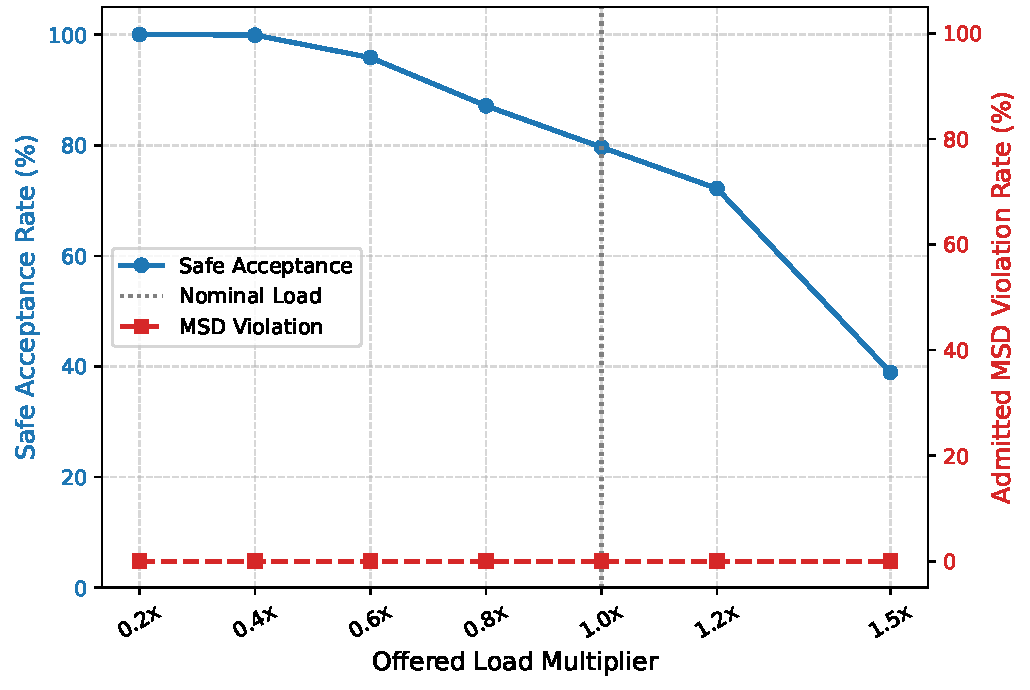
\includegraphics[width=\linewidth]{Figs/VN_load_sweep.pdf}
    \caption{Load sweep simulation on the Vietnam backbone under varying arrival rates. All algorithms preserve zero admitted MSD violations, while HARP achieves higher acceptance rates under heavy load.}
    \label{fig:vn_load_sweep}
\end{figure}

\subsection{Simulation Results across Distributed Topologies}
\label{subsec:simulation_results}

\autoref{tab:simulation_acceptance_summary} summarizes the request acceptance behavior across all stress scenarios. HARP consistently admits more useful requests than Greedy, DAI, and the deterministic SAF-H baseline in most stress settings. On the Vietnam backbone, HARP accepts \(17.89\% - 18.74\%\) of requests, compared with \(4.07\% - 4.29\%\) for Greedy and \(4.40\% - 4.43\%\) for DAI. On NSFNET, HARP reaches \(29.41\% - 31.51\%\), roughly four times the Greedy acceptance rate. GEANT2 provides the richest path diversity, and HARP achieves \(44.73\% - 49.52\%\), again substantially above both baselines.

SAF-H provides a stricter comparison because it enforces CPU, memory, and MSD feasibility before admission. Its behavior is therefore safer than Greedy and DAI, but it remains myopic: it selects the locally cheapest feasible service path without learning how current placements affect future residual headroom. HARP improves over SAF-H especially under bursty and chaotic workloads, where graph-aware policy learning helps preserve feasible placement--routing options for subsequent requests.

\begin{table}[t]
\centering
\caption{Stress simulation summary: acceptance rate across topologies and workloads (\%).}
\label{tab:simulation_acceptance_summary}
\renewcommand{\arraystretch}{1.15}
\scriptsize
\resizebox{\linewidth}{!}{
\begin{tabular}{llcccc}
\toprule
\textbf{Topology} & \textbf{Scenario} & \textbf{Greedy} & \textbf{DAI} & \textbf{SAF-H} & \textbf{HARP} \\
\midrule
Vietnam & Elephant & 4.07 $\pm$ 0.20 & 4.40 $\pm$ 0.20 & 16.27 $\pm$ 0.59 & \textbf{17.89} $\pm$ \textbf{0.67} \\
 & Burst surge & 4.29 $\pm$ 0.15 & 4.43 $\pm$ 0.80 & 17.47 $\pm$ 0.43 & \textbf{18.74} $\pm$ \textbf{0.51} \\
 & Chaos & 4.07 $\pm$ 0.20 & 4.40 $\pm$ 0.20 & 16.27 $\pm$ 0.59 & \textbf{17.89} $\pm$ \textbf{0.67} \\
\midrule
NSFNET & Elephant & 6.81 $\pm$ 0.67 & 6.41 $\pm$ 0.46 & \textbf{29.61} $\pm$ \textbf{0.36} & 29.41 $\pm$ 0.47 \\
 & Burst surge & 7.66 $\pm$ 0.45 & 6.45 $\pm$ 1.69 & \textbf{32.32} $\pm$ \textbf{0.50} & 31.51 $\pm$ 0.81 \\
 & Chaos & 6.81 $\pm$ 0.67 & 6.41 $\pm$ 0.46 & \textbf{29.61} $\pm$ \textbf{0.36} & 29.41 $\pm$ 0.47 \\
\midrule
GEANT2 & Elephant & 8.47 $\pm$ 0.91 & 8.14 $\pm$ 1.72 & 43.82 $\pm$ 0.86 & \textbf{44.73} $\pm$ \textbf{0.80} \\
 & Burst surge & 8.67 $\pm$ 0.61 & 9.21 $\pm$ 1.59 & 48.26 $\pm$ 0.64 & \textbf{49.52} $\pm$ \textbf{0.48} \\
 & Chaos & 8.47 $\pm$ 0.91 & 8.14 $\pm$ 1.72 & 43.82 $\pm$ 0.86 & \textbf{44.73} $\pm$ \textbf{0.80} \\
\bottomrule
\end{tabular}
}
\end{table}

The Vietnam results show the behavior of HARP under the most constrained topology. In Elephant stress, HARP increases acceptance from \(4.07\%\) to \(17.89\%\) compared with Greedy and reduces average latency on the accepted set. In Burst surge, HARP reaches \(18.74\%\), showing that the graph-aware policy is not merely conservative. It can find feasible placement--routing combinations that are missed by local or decoupled strategies. Chaos stress produces a similar acceptance rate to Elephant stress, which is expected because both scenarios combine large demands with difficult paths.

The NSFNET results follow the same trend. HARP accepts \(29.41\%\) of requests under Elephant and Chaos stress and \(31.51\%\) under Burst surge. The gain over Greedy remains close to a factor of four. This suggests that the policy is not exploiting only the specific geometry of the Vietnam topology. It benefits from graph-aware reasoning when the substrate contains different path structures and residual-capacity distributions.

GEANT2 produces the strongest acceptance results. The richer topology provides more alternative paths and therefore more opportunities for a graph-aware policy to find deployable actions. HARP accepts \(44.73\%\) of requests under Elephant and Chaos stress and \(49.52\%\) under Burst surge. Both Greedy and DAI remain below \(10\%\) in these scenarios. The gap indicates that HARP is not simply rejecting more aggressively; it is selecting from the feasible region more effectively.

The unsafe-candidate behavior must be interpreted carefully. In the algorithmic simulation, the reported pre-admission MSD-infeasible candidate accounting reflects the number of candidate decisions that become infeasible under severe stress, not necessarily requests admitted into a real data plane. For example, in the Vietnam stress scenarios, HARP reduces pre-admission MSD-infeasible candidate accounting from approximately \(95.6\%--96.3\%\) for the baselines to \(84.2\%--85.6\%\). The absolute value remains high because the workload is intentionally beyond safe capacity. The important point is that HARP shifts the candidate distribution toward safer and more useful decisions, while the runtime admission layer is responsible for ensuring that unsafe candidates do not become admitted data-plane actions.

\begin{figure}[t]
    \centering
    
\includegraphics[width=\linewidth]{figs/VN_burst.pdf}
    \caption{Vietnam backbone simulation under Burst surge. HARP improves acceptance under rapid admission pressure while reducing pre-admission MSD-infeasible candidate pressure relative to the baselines. These candidates are rejected before actuation and should not be interpreted as admitted data-plane violations.}
    \label{fig:vn_burst_result}
\end{figure}



\begin{figure}[t]
    \centering
    
\includegraphics[width=\linewidth]{figs/Geant2_burst.pdf}
    \caption{GEANT2 simulation under Burst surge. The richer topology provides more feasible alternatives, allowing HARP to achieve the strongest acceptance improvement.}
    \label{fig:geant_burst_result}
\end{figure}

% \begin{figure}[t]
% \centering
% \begin{tikzpicture}

% \pgfplotsset{
%     compactbar/.style={
%         ybar,
%         bar width=7pt,
%         bar shift=0pt,
%         width=0.47\columnwidth,
%         height=0.34\columnwidth,
%         enlarge x limits=0.25,
%         symbolic x coords={Traditional Greedy,Decoupled AI,HARP},
%         xtick=data,
%         xticklabel style={rotate=18, anchor=east, font=\tiny},
%         ymajorgrids=true,
%         grid style={gray!20},
%         tick label style={font=\tiny},
%         label style={font=\tiny},
%         title style={font=\bfseries\tiny},
%         nodes near coords,
%         every node near coord/.append style={font=\tiny, yshift=1pt},
%         axis line style={black},
%         tick style={black}
%     }
% }

% \begin{groupplot}[
%     group style={
%         group size=2 by 3,
%         horizontal sep=0.18cm,
%         vertical sep=0.42cm
%     }
% ]

% % ---------------- Acceptance Rate ----------------
% \nextgroupplot[
%     compactbar,
%     title={Acceptance Rate (\%)},
%     ymin=0,
%     ymax=36.5,
%     ytick={0,5,10,15,20,25,30,35}
% ]
% \addplot[fill=orange!85, draw=none] coordinates {(Traditional Greedy,8.8)};
% \addplot[fill=blue!70, draw=none] coordinates {(Decoupled AI,6.0)};
% \addplot[fill=red!75, draw=none] coordinates {(HARP,30.0)};

% % ---------------- MSD Violation Rate ----------------
% \nextgroupplot[
%     compactbar,
%     title={MSD Violation Rate (\%)},
%     ymin=0,
%     ymax=114,
%     ytick={0,20,40,60,80,100}
% ]
% \addplot[fill=orange!85, draw=none] coordinates {(Traditional Greedy,91.2)};
% \addplot[fill=blue!70, draw=none] coordinates {(Decoupled AI,94.0)};
% \addplot[fill=red!75, draw=none] coordinates {(HARP,64.5)};

% % ---------------- SLA Violation Rate ----------------
% \nextgroupplot[
%     compactbar,
%     title={SLA Violation Rate (\%)},
%     ymin=0,
%     ymax=1.82,
%     ytick={0,0.25,0.50,0.75,1.00,1.25,1.50,1.75}
% ]
% \addplot[fill=orange!85, draw=none] coordinates {(Traditional Greedy,0.0)};
% \addplot[fill=blue!70, draw=none] coordinates {(Decoupled AI,0.1)};
% \addplot[fill=red!75, draw=none] coordinates {(HARP,1.4)};

% % ---------------- Average Latency ----------------
% \nextgroupplot[
%     compactbar,
%     title={Average Latency (ms)},
%     ymin=0,
%     ymax=8.4,
%     ytick={0,1,2,3,4,5,6,7,8}
% ]
% \addplot[fill=orange!85, draw=none] coordinates {(Traditional Greedy,3.7)};
% \addplot[fill=blue!70, draw=none] coordinates {(Decoupled AI,2.5)};
% \addplot[fill=red!75, draw=none] coordinates {(HARP,6.8)};

% % ---------------- M/G/1 Queue Latency ----------------
% \nextgroupplot[
%     compactbar,
%     title={M/G/1 Queue Latency (ms)},
%     ymin=0,
%     ymax=0.465,
%     ytick={0,0.1,0.2,0.3,0.4}
% ]
% \addplot[fill=orange!85, draw=none] coordinates {(Traditional Greedy,0.1)};
% \addplot[fill=blue!70, draw=none] coordinates {(Decoupled AI,0.1)};
% \addplot[fill=red!75, draw=none] coordinates {(HARP,0.3)};

% % ---------------- Average Reward ----------------
% \nextgroupplot[
%     compactbar,
%     title={Average Reward},
%     ymin=-15.5,
%     ymax=16,
%     ytick={-15,-10,-5,0,5,10,15},
%     every node near coord/.append style={font=\tiny}
% ]
% \addplot[
%     fill=orange!85,
%     draw=none,
%     nodes near coords,
%     every node near coord/.append style={anchor=north, yshift=-1pt}
% ] coordinates {(Traditional Greedy,-7.5)};

% \addplot[
%     fill=blue!70,
%     draw=none,
%     nodes near coords,
%     every node near coord/.append style={anchor=north, yshift=-1pt}
% ] coordinates {(Decoupled AI,-12.0)};

% \addplot[
%     fill=red!75,
%     draw=none,
%     nodes near coords,
%     every node near coord/.append style={anchor=south, yshift=1pt}
% ] coordinates {(HARP,12.6)};

% \end{groupplot}

% \end{tikzpicture}
%     \caption{GEANT2 simulation under Burst surge. The richer topology provides more feasible alternatives, allowing HARP to achieve the strongest acceptance improvement.}
%     \label{fig:geant_burst_result}
% \end{figure}

The latency and reward results are consistent with the acceptance results. In the Vietnam stress scenarios, HARP keeps the average latency of accepted requests below the corresponding baseline values. On NSFNET and GEANT2, latency should be read together with acceptance because baselines often accept a much smaller and easier subset of requests. A method that accepts only a few short-path flows may report low latency while failing to serve most demand. HARP improves the useful admitted set while maintaining better reward trends, which is the more relevant criterion under stress.

    \subsection{Ablation Study}
\label{subsec:ablation_study}

The ablation study is designed to answer EQ3 by isolating the main design choices behind HARP: graph-aware topology encoding, hard action masking, adaptive soft-constraint control, and proactive migration. All ablation variants follow the same workload generator, topology settings, and safety metrics as the full HARP policy. The study is organized in two parts. Section~\ref{subsubsec:ablation_vietnam} uses the Vietnam topology to perform a detailed architectural component analysis, isolating individual failure modes. Section~\ref{subsubsec:pareto_tradeoffs} extends the analysis to NSFNET and GEANT2, examining the multi-dimensional trade-off landscape across the design variants.

The variants in \autoref{tab:ablation_variants} separate the failure modes targeted by HARP. \textbf{PPO-MLP} tests whether replacing the graph-attention encoder with a flat state representation weakens topology-dependent placement and routing. \textbf{HARP w/o masking} and \textbf{HARP-SoftMSD} test whether hardware feasibility can be safely handled after policy selection or through a reward penalty. \textbf{HARP w/o adaptive penalty} evaluates whether fixed reward weights are sufficient under bursty service-level pressure. \textbf{HARP w/o migration} isolates the contribution of proactive migration under overload and DDoS-triggered make-before-break scenarios.

This component analysis also clarifies the difference between algorithmic quality and operational safety. A variant without hard masking may appear to improve raw acceptance if unsafe actions are counted as accepted candidates, but such decisions are not deployable on an SRv6/P4 data plane. For this reason, the ablation results should be interpreted primarily through safe acceptance, unsafe candidate rate, and admitted MSD violation rate rather than raw acceptance alone. The expected behavior of a hardware-safe orchestrator is not to maximize admission at any cost, but to admit only those actions that can be translated into feasible cloud-native lifecycle and programmable data-plane operations.

\subsubsection{Architectural Ablation on Vietnam Backbone}
\label{subsubsec:ablation_vietnam}
\begin{table}[t]
\centering
\caption{Ablation results on the Vietnam topology. All percentage columns are reported in \%.}
\label{tab:vietnam_ablation_summary}
\renewcommand{\arraystretch}{1.12}
\setlength{\tabcolsep}{2pt}
\scriptsize
\resizebox{\linewidth}{!}{
\begin{tabular}{llrrrrr}
\toprule
\textbf{Scen.} & \textbf{Var.} &
\makecell{\textbf{Safe}\\\textbf{acc.}} &
\makecell{\textbf{Pre-adm.}\\\textbf{MSD}} &
\makecell{\textbf{Adm.}\\\textbf{MSD}} &
\textbf{SLA} &
\makecell{\textbf{Lat.}\\\textbf{ms}} \\
\midrule
\multirow{6}{*}{Uniform}
& Full & \textbf{18.90} $\pm$ \textbf{0.45} & 81.05 $\pm$ 0.52 & \textbf{0.00} $\pm$ \textbf{0.00} & \textbf{0.00} $\pm$ \textbf{0.00} & 1.44 $\pm$ 0.09 \\
& MLP & 17.47 $\pm$ 0.51 & 82.51 $\pm$ 0.50 & \textbf{0.00} $\pm$ \textbf{0.00} & \textbf{0.00} $\pm$ \textbf{0.00} & 3.43 $\pm$ 0.15 \\
& NoMask & 18.59 $\pm$ 0.50 & 81.11 $\pm$ 0.62 & \textbf{0.00} $\pm$ \textbf{0.00} & \textbf{0.00} $\pm$ \textbf{0.00} & \textbf{0.78} $\pm$ \textbf{0.06} \\
& NoMask+U & 4.99 $\pm$ 0.54 & 91.01 $\pm$ 4.33 & 23.56 $\pm$ 1.56 & \textbf{0.00} $\pm$ \textbf{0.00} & 4.37 $\pm$ 0.12 \\
& SoftMSD & 1.39 $\pm$ 0.22 & 97.39 $\pm$ 0.73 & 34.53 $\pm$ 0.80 & 0.03 $\pm$ 0.04 & 2.53 $\pm$ 0.16 \\
& NoAdapt & 16.48 $\pm$ 0.40 & 83.48 $\pm$ 0.42 & \textbf{0.00} $\pm$ \textbf{0.00} & \textbf{0.00} $\pm$ \textbf{0.00} & 1.73 $\pm$ 0.43 \\
\midrule
\multirow{6}{*}{Bursty}
& Full & \textbf{18.74} $\pm$ \textbf{0.51} & 81.25 $\pm$ 0.53 & \textbf{0.00} $\pm$ \textbf{0.00} & \textbf{0.00} $\pm$ \textbf{0.00} & 0.87 $\pm$ 0.13 \\
& MLP & 17.72 $\pm$ 0.38 & 82.28 $\pm$ 0.38 & \textbf{0.00} $\pm$ \textbf{0.00} & \textbf{0.00} $\pm$ \textbf{0.00} & 3.74 $\pm$ 0.08 \\
& NoMask & 13.77 $\pm$ 1.47 & 86.19 $\pm$ 1.46 & \textbf{0.00} $\pm$ \textbf{0.00} & \textbf{0.00} $\pm$ \textbf{0.00} & \textbf{0.26} $\pm$ \textbf{0.05} \\
& NoMask+U & 4.41 $\pm$ 0.34 & 93.59 $\pm$ 1.17 & 31.78 $\pm$ 1.06 & 0.01 $\pm$ 0.01 & 4.08 $\pm$ 0.10 \\
& SoftMSD & 1.58 $\pm$ 0.14 & 98.29 $\pm$ 0.23 & 34.38 $\pm$ 1.06 & \textbf{0.00} $\pm$ \textbf{0.00} & 2.84 $\pm$ 0.10 \\
& NoAdapt & 16.51 $\pm$ 0.75 & 83.49 $\pm$ 0.75 & \textbf{0.00} $\pm$ \textbf{0.00} & \textbf{0.00} $\pm$ \textbf{0.00} & 0.93 $\pm$ 0.18 \\
\midrule
\multirow{6}{*}{Heavy-tail}
& Full & \textbf{17.89} $\pm$ \textbf{0.67} & 81.97 $\pm$ 0.65 & \textbf{0.00} $\pm$ \textbf{0.00} & \textbf{0.00} $\pm$ \textbf{0.00} & 1.88 $\pm$ 0.16 \\
& MLP & 16.57 $\pm$ 0.53 & 83.43 $\pm$ 0.53 & \textbf{0.00} $\pm$ \textbf{0.00} & \textbf{0.00} $\pm$ \textbf{0.00} & 3.29 $\pm$ 0.19 \\
& NoMask & 17.15 $\pm$ 0.74 & 82.26 $\pm$ 0.70 & \textbf{0.00} $\pm$ \textbf{0.00} & \textbf{0.00} $\pm$ \textbf{0.00} & \textbf{1.04} $\pm$ \textbf{0.11} \\
& NoMask+U & 3.89 $\pm$ 0.31 & 94.04 $\pm$ 1.25 & 23.22 $\pm$ 0.62 & 0.07 $\pm$ 0.05 & 4.68 $\pm$ 0.17 \\
& SoftMSD & 1.12 $\pm$ 0.15 & 98.19 $\pm$ 0.77 & 33.57 $\pm$ 0.41 & 0.03 $\pm$ 0.03 & 2.25 $\pm$ 0.03 \\
& NoAdapt & 16.06 $\pm$ 0.43 & 83.93 $\pm$ 0.43 & \textbf{0.00} $\pm$ \textbf{0.00} & \textbf{0.00} $\pm$ \textbf{0.00} & 1.71 $\pm$ 0.26 \\
\bottomrule
\end{tabular}
}
\end{table}

Table~\ref{tab:vietnam_ablation_summary} reports the ablation results on the Vietnam backbone topology. The full HARP policy achieves the highest safe acceptance across all three workload scenarios while maintaining \(0.0\%\) admitted MSD violations. The following paragraphs examine each ablation component in turn.

\paragraph{Graph-attention topology encoding (PPO-MLP)}
Replacing the graph-attention encoder with a flat MLP state encoder degrades both safe acceptance and latency. The MLP variant loses \(1.0\)--\(1.4\) percentage points of safe acceptance and significantly increases latency across all three scenarios (e.g., \(3.29\)~ms vs.\ \(1.88\)~ms under heavy-tail). The latency increase indicates that the flat encoder tends to select placement--routing pairs with longer or more congested paths, because it cannot reason about the topological distance between source, placement node, and destination.

\paragraph{Hard action masking (NoMask)}
Disabling the hard action mask while retaining runtime admission validation produces results that depend on topology scale. On Vietnam (\(N{=}10\), action space \(N^2{=}100\)), the NoMask variant achieves safe acceptance close to full HARP (\(17.15\%\) vs.\ \(17.89\%\) under heavy-tail) with \(0.0\%\) admitted MSD violations, because the runtime admission layer successfully filters infeasible candidates. However, as shown in the trade-off analysis of Section~\ref{subsubsec:pareto_tradeoffs}, this masking advantage becomes critical on larger topologies where the expanded action space prevents reward-based learning from discovering feasible placement--routing pairs.

\paragraph{Two-layer safety separation (NoMask vs.\ NoMask+U)}
The comparison between NoMask and NoMask+U isolates the contribution of the runtime admission layer independently from the policy-side mask. NoMask maintains \(0.0\%\) admitted MSD violations because the admission layer catches infeasible outputs; NoMask+U, which removes this safety net, permits \(23.22\%\)--\(31.78\%\) of accepted requests to carry MSD violations. This demonstrates that HARP's safety architecture relies on two complementary layers: the policy-side mask reduces the probability of sampling infeasible actions during inference, and the runtime admission check rejects any remaining violations before actuation. This two-layer design is particularly relevant for SRv6/P4 orchestration, where a single admitted MSD violation translates to a non-parseable packet header rather than a degraded but recoverable service outcome.

\paragraph{Hard constraint vs.\ reward penalty (SoftMSD)}
The HARP-SoftMSD variant converts MSD feasibility from a hard mask condition to a reward penalty term. The results are unambiguous: SoftMSD produces admitted MSD violation rates of \(33.57\%\)--\(34.53\%\), while safe acceptance collapses to \(1.12\%\)--\(1.58\%\). This dual failure occurs because the reward penalty creates a conflict between admission incentive and safety cost. The policy learns to avoid most MSD violations by becoming overly conservative, but the residual violation rate remains far too high for data-plane deployment. This reinforces a design principle: SRv6/P4 parser-depth constraints are binary pass-or-fail conditions at the hardware level and should not be treated as soft optimization targets.

\paragraph{Adaptive penalty control (NoAdapt)}
Replacing the adaptive SLA and migration penalty with fixed reward weights produces a variant that remains deployable---admitted MSD violations stay at \(0.0\%\)---but loses \(1.8\)--\(2.4\) percentage points of safe acceptance across scenarios (e.g., \(16.06\%\) vs.\ \(17.89\%\) under heavy-tail) and increases latency modestly. The adaptive penalty mechanism is therefore not critical for safety but necessary for sustained service-level quality under varying load patterns.

\paragraph{Vietnam ablation summary}
On the Vietnam backbone, the ablation evidence supports the combination of mechanisms used by full HARP. Hard action masking is a prerequisite for safety: converting MSD to a soft penalty fails to achieve the elimination guarantee required by SRv6/P4 hardware. The two-layer safety architecture provides defense in depth against MSD violations. The graph-attention encoder provides topology-dependent placement quality that a flat representation cannot match, and adaptive penalty control improves SLA compliance without affecting safety. The next section examines whether these component effects generalize---and how they interact with topology scale---on the larger NSFNET and GEANT2 networks.

\subsubsection{Architectural Trade-offs and Pareto Optimality on Large-scale Topologies}
\label{subsubsec:pareto_tradeoffs}

The Vietnam ablation in Section~\ref{subsubsec:ablation_vietnam} evaluates each design component in isolation. On larger topologies, however, the relevant question shifts from ``which component matters?'' to ``how do the design choices interact in a multi-dimensional trade-off space?'' A variant that appears competitive on one metric (e.g., safe acceptance) may simultaneously degrade others (e.g., latency, SLA compliance, or action stability). To capture these interactions, \autoref{fig:pareto_design_space} projects the six ablation variants onto three pairwise trade-off planes---SLA compliance vs.\ acceptance, routing quality vs.\ acceptance, and action stability vs.\ acceptance---and identifies the Pareto-optimal operating points on both NSFNET (14 nodes, $N^2{=}196$ actions) and GEANT2 (23 nodes, $N^2{=}529$ actions). Each marker represents one design variant averaged across all three traffic scenarios (Uniform, Bursty, Heavy-tail), with cross-scenario error bars; per-scenario values are shown as faint background markers.

\begin{figure*}[t]
    \centering
    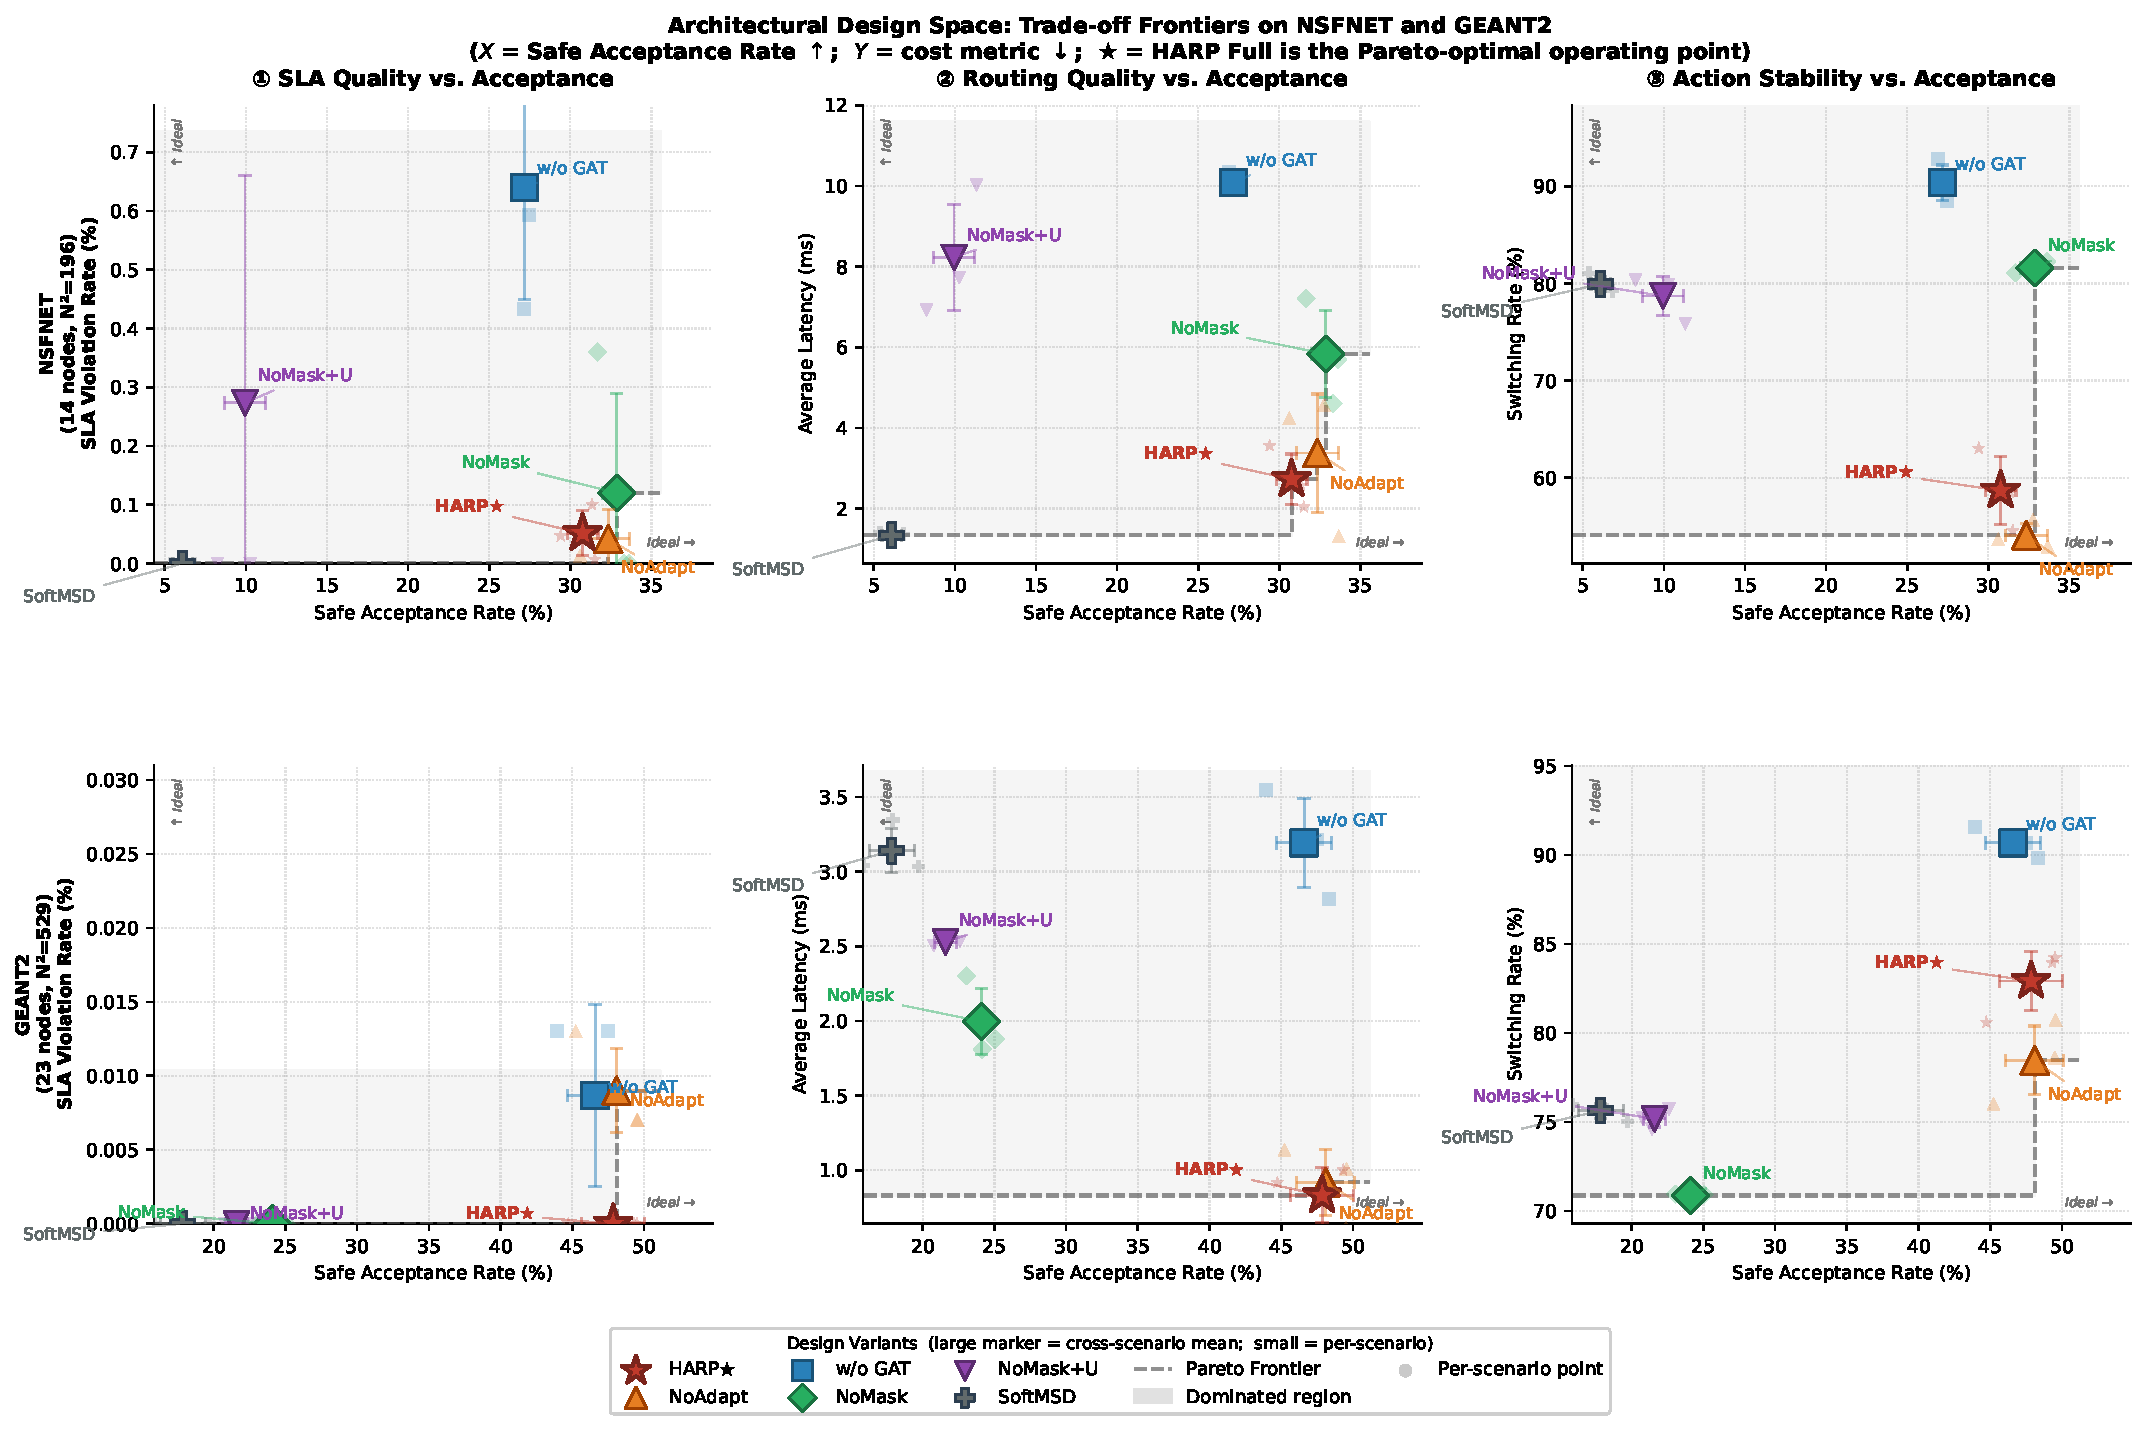
\includegraphics[width=\linewidth]{Figs/pareto_design_space.pdf}
    \caption{Architectural design-space trade-offs on NSFNET and GEANT2. Each column shows a pairwise trade-off between Safe Acceptance Rate ($\uparrow$) and a cost metric ($\downarrow$). Large markers are cross-scenario means; small markers are per-scenario values. The dashed line marks the Pareto frontier; the shaded region contains dominated design points. HARP~Full~($\bigstar$) is Pareto-optimal or near-optimal across all six subplots.}
    \label{fig:pareto_design_space}
\end{figure*}

\paragraph{Trade-off~\ding{172}: SLA compliance vs.\ acceptance}
The leftmost column of \autoref{fig:pareto_design_space} plots SLA violation rate against safe acceptance. On NSFNET, the PPO-MLP variant is the worst-performing point: it reaches only $27.2\%$ safe acceptance while incurring the highest SLA violation rate ($0.64\%$). Full HARP achieves $30.8\%$ acceptance with SLA violations near zero ($0.05\%$), and the NoAdapt variant reaches $32.3\%$ acceptance but at a comparable SLA cost ($0.04\%$). On GEANT2, all variants achieve SLA violation rates below $0.01\%$, reflecting the richer path diversity of the 23-node topology. However, unsafe variants (NoMask, NoMask+U, SoftMSD) cluster at the left side with safe acceptance below $25\%$, while Full HARP and NoAdapt dominate the right side near $48\%$. This confirms that the adaptive penalty mechanism is primarily valuable on medium-scale topologies like NSFNET, where path scarcity creates SLA pressure; on GEANT2, the topological redundancy absorbs most SLA stress even without adaptive control.

\paragraph{Trade-off~\ding{173}: routing quality vs.\ acceptance}
The center column reveals the most dramatic separation. On NSFNET, PPO-MLP reaches $10.08$~ms average latency---$3.7{\times}$ higher than Full HARP's $2.73$~ms---while also achieving lower acceptance. The flat encoder cannot reason about path lengths or congestion patterns, so it systematically selects placement--routing pairs with longer segment lists. On GEANT2, the latency gap narrows but remains significant: PPO-MLP averages $3.19$~ms versus $0.83$~ms for Full HARP. Critically, Full HARP occupies the lower-right corner of both subplots---high acceptance \emph{and} low latency---demonstrating that the graph-attention encoder breaks the usual acceptance--latency trade-off rather than merely shifting the operating point along it.

\paragraph{Trade-off~\ding{174}: action stability vs.\ acceptance}
The rightmost column plots switching rate (the fraction of decisions that change the placement or routing of an existing flow) against safe acceptance. On NSFNET, PPO-MLP exhibits the highest switching rate ($90.4\%$) with the lowest acceptance, indicating chaotic decision-making: the flat policy frequently re-routes flows without improving admission outcomes. Full HARP reduces switching to $58.7\%$ while maintaining competitive acceptance, reflecting more purposeful re-routing decisions. On GEANT2, Full HARP's switching rate ($82.9\%$) is higher than NoAdapt's ($78.5\%$) and NoMask's ($70.9\%$), but this is not instability: the GAT-driven policy actively exploits the richer path alternatives of the 23-node topology, re-routing flows to maintain acceptance under load pressure. The lower switching rate of NoMask on GEANT2 is a symptom of policy collapse---the agent converges to a single repeated action and ceases meaningful exploration---rather than stability.

\paragraph{Pareto optimality}
Across all six subplots in \autoref{fig:pareto_design_space}, Full HARP consistently occupies the Pareto frontier or lies within one standard deviation of it. No other variant achieves simultaneously higher acceptance, lower latency, lower SLA violations, and more purposeful switching behavior. The unsafe variants (NoMask+U, SoftMSD) are deeply dominated: they sacrifice both acceptance and safety, landing in the shaded region on every trade-off plane. The NoAdapt variant is the closest competitor on acceptance, but it concedes measurable ground on SLA compliance (NSFNET) and latency (both topologies). The PPO-MLP variant, lacking topology awareness, is dominated on every dimension across both topologies. These results establish that the full HARP design is not merely one point among many reasonable alternatives, but the Pareto-optimal operating point in the architectural design space across multiple operational dimensions and topology scales.

\subsection{Hardware-in-the-Loop Testbed Validation}
\label{subsec:testbed_validation}

The hardware-in-the-loop testbed evaluates whether the AIO-Mesh control loop can preserve data-plane safety after the algorithmic decision stage. The testbed uses five scenarios: Normal load, Elephant heavy-tail, Topology and physics stress, DDoS with make-before-break triggering, and Chaos. These scenarios differ from the simulation benchmark in one important way: unsafe choices are not counted as admitted service actions. The runtime can reject them as \texttt{NO\_SAFE\_ACTION}, while the P4 data plane still exposes MSD-drop counters as a final verification signal.

Table~\ref{tab:testbed_results} reports acceptance and admitted MSD violation rates. HARP and the Hybrid runtime maintain \(0.0\%\) admitted MSD violations in all scenarios. This is the core deployment result. Under Normal load, HARP, Hybrid runtime, Heuristic, and Greedy all accept \(100.0\%\) of requests without admitted MSD violations, while DAI already records violations. Under Elephant heavy-tail, HARP accepts \(71.0\%\) with no admitted MSD violations, while Greedy and DAI accept fewer requests and produce admitted MSD violations. Under Topology and physics stress, Greedy appears to match the HARP acceptance rate, but it does so with \(78.8\%\) admitted MSD violations. This result shows why raw acceptance is not a sufficient metric for SRv6/P4 orchestration.

\begin{table}[t]
\centering
\caption{Hardware-in-the-loop testbed results: acceptance rate / admitted MSD violation rate.}
\label{tab:testbed_results}
\renewcommand{\arraystretch}{1.08}
\setlength{\tabcolsep}{2pt}
\scriptsize
\resizebox{\linewidth}{!}{
\begin{tabular}{@{}lccccc@{}}
\toprule
\textbf{Algorithm} &
\makecell{\textbf{Normal}} &
\makecell{\textbf{Elephant}} &
\makecell{\textbf{Topo}\\\textbf{stress}} &
\makecell{\textbf{DDoS}\\\textbf{MBB}} &
\textbf{Chaos} \\
\midrule
\textbf{HARP}  & 100.0 / 0.0 & 71.0 / 0.0 & 21.2 / 0.0 & 23.0 / 0.0 & 10.0 / 0.0 \\
Hybrid runtime & 100.0 / 0.0 & \textbf{75.3} / 0.0 & 21.2 / 0.0 & 24.8 / 0.0 & 8.3 / 0.0 \\
Heuristic      & 100.0 / 0.0 & 65.6 / 0.0 & 20.3 / 0.0 & 22.1 / 0.0 & 7.9 / 0.0 \\
Greedy         & 100.0 / 0.0 & 59.1 / 19.4 & 21.2 / 78.8 & \textbf{25.7} / 69.0 & 7.9 / 79.2 \\
DAI   & 94.1 / 5.9  & 52.7 / 22.6 & 9.3 / 90.7  & 18.6 / 77.9 & 5.8 / 81.3 \\
\bottomrule
\end{tabular}
}
\end{table}

The DDoS and make-before-break scenario is particularly informative. Greedy reaches \(25.7\%\) acceptance, slightly higher than HARP, but incurs \(69.0\%\) admitted MSD violations. HARP accepts \(23.0\%\) with zero admitted MSD violations, while the Hybrid runtime accepts \(24.8\%\) with zero admitted violations. This confirms the intended role of the hybrid design: inexpensive heuristic decisions can be used when safe, while the learned policy and admission layer prevent unsafe actuation under stress.

The Chaos scenario is the saturation case. HARP accepts \(10.0\%\) of requests, Hybrid runtime accepts \(8.3\%\), and the baselines remain below or near that range. The important result is not high acceptance; the workload is intentionally beyond safe capacity. The important result is that HARP, Hybrid runtime, and the safety-preserving heuristic maintain \(0.0\%\) admitted MSD violations, while Greedy and DAI produce \(79.2\%\) and \(81.3\%\) admitted MSD violations, respectively. In this regime, safe rejection is the correct operational behavior.

\begin{figure*}[t]
    \centering
    \includegraphics[width=\linewidth]{figs/testbed.pdf}
    \caption{Hardware-in-the-loop testbed used to validate the AIO-Mesh control loop with MicroK8s, Tekton, Mininet, BMv2 P4 switches, SRv6 steering, and runtime admission control.}
    \label{fig:testbed_architecture_eval}
\end{figure*}

The testbed results clarify the relationship between the simulation and deployment evaluations. Simulation exposes the policy's behavior under stress and reports unsafe candidate pressure. The testbed verifies that unsafe candidates are converted into explicit admission rejections before they become data-plane actions. This is the main reason why the testbed can report zero admitted MSD violations even when the algorithmic stress benchmark still shows high unsafe-candidate rates.

\subsection{Make-Before-Break Migration Behavior}
\label{subsec:mbb_evaluation}

AIO-Mesh implements make-before-break migration as a controlled orchestration sequence. The replacement VNF is created first, Kubernetes readiness is verified, the new endpoint is translated into an SRv6-safe service path, the controller installs the steering state, and only then is the old VNF eligible for removal. This ordering prevents the orchestrator from deleting a working function before traffic can reach the replacement.

The DDoS and make-before-break scenario exercises this path by generating overload conditions that trigger the migration branch of the control loop. The Hybrid runtime records migration triggers under this scenario and maintains zero admitted MSD violations. This validates the control-plane sequencing and safety gating required for proactive migration.

We do not claim full zero-downtime migration solely from the orchestration sequence. A strict zero-downtime claim requires packet-level evidence, such as continuous TCP sequence/acknowledgement traces or packet-capture validation showing that the old path remains available until the new SRv6 steering state is active. The current evaluation therefore supports the claim that AIO-Mesh implements a safety-preserving make-before-break control sequence, while packet-continuity validation is left as an explicit follow-up measurement.

\subsection{Operational Overhead and Scalability}
\label{subsec:overhead_scalability}
AIO-Mesh is designed for online orchestration, so its runtime overhead must be interpreted at the level of the control loop. The main costs arise from state construction, graph-policy inference, feasibility-mask construction, admission validation, SRv6/P4 steering, and cloud-native lifecycle actuation. These costs have different operational meanings. State construction, HARP inference, mask construction, and admission validation determine how quickly the controller can make an online admission or steering decision. In contrast, SRv6/P4 rule installation, VNF deployment, and make-before-break migration are actuator-side costs that depend on the controller implementation, workflow engine, container runtime, and programmable-data-plane backend.

For the evaluated topologies, the policy-side path remains lightweight because the substrate graph is small compared with the number of traffic flows. For a graph with (N) nodes, (E) edges, (K) attention heads, and hidden dimension (F), the dominant cost of one graph-attention layer is
\begin{equation}
\mathcal{O}(N F^2 K + E F K).
\end{equation}
This cost is practical for backbone-scale orchestration because (N) and (E) describe the infrastructure substrate rather than individual traffic flows. In addition, stable topology snapshots allow candidate paths and SID-depth metadata to be cached, so feasibility-mask construction mainly requires checking residual CPU, memory, and MSD constraints against the current request and telemetry state.

The larger operational delay is expected to come from actuation rather than policy inference. Creating or migrating a VNF through Kubernetes/Tekton involves scheduling, image handling, readiness checks, service exposure, and workflow coordination. Similarly, SRv6/P4 steering requires rule generation, controller communication, and confirmation from the data-plane interface. These delays should not be attributed to the graph policy itself. AIO-Mesh therefore separates decision latency from actuation latency: the former determines whether the system can perform online admission control, while the latter determines how quickly an admitted decision becomes effective in the infrastructure.

This separation is important for interpreting the hardware-in-the-loop results. The evaluation demonstrates that AIO-Mesh can embed a learned policy inside a cloud-native control loop and prevent hardware-infeasible actions from becoming admitted data-plane behavior. It does not claim line-rate forwarding performance or production-grade migration latency. Such measurements require deployment on production programmable targets, such as ASIC-based P4 switches, smartNICs, or DPUs, together with controller-specific latency instrumentation. The current prototype instead validates the operational feasibility of the control loop, the scalability of graph-policy inference for the evaluated substrate sizes, and the correctness of fail-closed admission semantics under stress.


\subsection{Discussion}
\label{subsec:evaluation_discussion}

The evaluation supports four observations.

First, graph-aware hardware-safe policy selection improves useful admission under stress. Across Vietnam, NSFNET, and GEANT2, HARP consistently improves over Greedy and DAI and remains stronger than the hardware-aware SAF-H baseline in the most dynamic stress scenarios. The gain is largest in topologies with richer path diversity, such as GEANT2, where the graph-aware policy has more feasible alternatives to exploit.

Second, raw acceptance is not a reliable metric for programmable-data-plane SFC orchestration. A baseline can accept many requests by ignoring MSD constraints, but those requests are not deployable. The testbed results show this clearly: Greedy appears competitive in some scenarios if only acceptance is considered, but it produces high admitted MSD violation rates under stress. HARP and the Hybrid runtime accept fewer requests in saturated cases, but the accepted requests remain hardware-safe.

Third, the ablation design clarifies why HARP is structured as a combination of topology encoding, hard masking, adaptive penalties, and migration support. On the Vietnam backbone, each component is isolated to identify its specific failure mode: the hard mask prevents non-deployable actions, the graph encoder improves placement quality, and the adaptive penalty sustains SLA compliance. On the larger NSFNET and GEANT2 topologies, the Pareto trade-off analysis (\\autoref{fig:pareto_design_space}) further demonstrates that Full HARP is the Pareto-optimal operating point across SLA compliance, routing quality, and action stability simultaneously---no other design variant achieves comparable performance on all dimensions.

Fourth, AIOps runtime design is part of the contribution. The learned policy is not evaluated only as an offline optimizer. It is embedded in a control loop that performs state construction, inference, hard-feasibility masking, admission handling, cloud-native lifecycle actuation, SRv6/P4 steering, and feedback monitoring. This integration is what turns a graph RL policy into an operational service-chain orchestrator.

Several limitations remain. The programmable data plane is evaluated with BMv2 rather than a production ASIC target such as Tofino. BMv2 is sufficient for validating parser-depth logic and control-plane behavior, but it does not provide line-rate hardware performance. The traffic workloads are stress-oriented and synthetic; production traces would strengthen the external validity of the evaluation. The forecasting adapter is treated as an operational trigger and not as a separately validated prediction model. Finally, make-before-break migration sequencing is implemented, but zero-downtime migration should only be claimed after packet-level continuity evidence is collected.

These limitations do not weaken the main safety result. The key claim of AIO-Mesh is not that every request can be admitted under saturation, or that migration is already proven zero-downtime. The key claim is that a learned AIOps policy can be embedded into a cloud-native SRv6/P4 orchestration loop while preventing hardware-infeasible actions from becoming admitted data-plane behavior.

\section{Conclusion}
\label{sec:conclusion}

This paper introduced \textbf{AIO-Mesh}, a hardware-safe AIOps orchestration framework for cloud-native service function chains over programmable data planes. The motivation behind AIO-Mesh is that learned orchestration policies cannot be treated as offline optimizers when their outputs directly affect service placement, traffic steering, and programmable data-plane behavior. In SRv6/P4-based service chaining, a decision that appears efficient at the logical graph level may still be non-deployable if the resulting SID stack exceeds the parser-depth capability of the forwarding profile. This makes hardware safety a first-class orchestration requirement rather than a secondary optimization preference.

At the core of AIO-Mesh, we proposed \textbf{HARP}, a hardware-aware reinforcement policy for joint placement, routing, and proactive migration. HARP combines graph-attention-based topology encoding, masked policy optimization, adaptive penalties for soft operational objectives, and smart admission control. The key design principle is the separation between hard deployability constraints and soft performance objectives. CPU, memory, and SRv6 MSD feasibility are enforced through action masking and admission control before actuation, while latency, migration cost, and SLA pressure are handled through the reward function. This design prevents hardware-infeasible policy outputs from being converted into data-plane actions.

The evaluation shows that HARP improves useful admission under stress-oriented workloads across multiple topologies, including the Vietnam backbone, NSFNET, and GEANT2. More importantly, the hardware-in-the-loop testbed demonstrates that AIO-Mesh can preserve admission safety when the learned policy is embedded in an operational control loop. By integrating telemetry-driven state construction, policy inference, safety validation, Kubernetes/Tekton-based VNF lifecycle control, SRv6/P4 steering, and runtime feedback, AIO-Mesh converts unsafe candidates into explicit \texttt{NO\_SAFE\_ACTION} decisions rather than allowing them to become admitted MSD violations. This distinction is essential for evaluating service-chain orchestration under programmable data-plane constraints: lower acceptance under saturation can be the correct behavior if the remaining requests are not safely deployable.

The work also clarifies the boundary of the current prototype. The programmable data plane is validated with BMv2 rather than a production ASIC target, and the stress workloads are synthetic rather than derived from production traces. The make-before-break migration sequence is implemented as a controlled actuation workflow, but a strict zero-downtime claim requires packet-level continuity evidence. The forecasting component is treated as an operational trigger rather than as an independently optimized prediction model. These limitations are intentional in the current scope, where the primary focus is on hardware-safe AIOps orchestration and admission correctness.

Future work will extend AIO-Mesh in four directions. First, deployment on production programmable targets such as Tofino-class switches or smartNIC/DPUs would allow parser-depth enforcement, steering latency, and throughput behavior to be evaluated at line rate. Second, the policy lifecycle can be expanded into a fuller MLOps pipeline with model versioning, rollback, drift monitoring, and controlled retraining. Third, cross-topology transfer and domain adaptation should be studied so that a policy trained on one substrate can generalize to other regional or edge-cloud infrastructures with minimal retraining. Finally, packet-level validation should be added to quantify service continuity during make-before-break migration. Together, these extensions would move AIO-Mesh from a validated research prototype toward an operational AIOps substrate for hardware-safe service orchestration in future cloud-native infrastructures.


\section*{Declaration of Competing Interest}
\noindent The authors declare that they have no known competing financial interests or personal relationships that could have appeared to influence the work reported in this paper.


\section*{Funding}
This work was supported by the Ministry of Science and Technology of Vietnam under the National Science and Technology Program, project code KC-4.0-56/19-30.

\section*{Data and Code Availability}
The simulation scenarios, topology descriptions, workload configurations, testbed scripts, Mininet/BMv2 configuration, SRv6/P4 steering scripts, Tekton pipeline definitions, and evaluation logs used in this study will be made available upon publication to support reproducibility. An anonymized supplementary package containing configuration files, workload generators, and raw evaluation logs can be provided during review upon reasonable request.

\section*{Declaration of Generative AI and AI-Assisted Technologies in the Writing Process}
During the preparation of this work, the authors used generative AI and AI-assisted technologies to refine the scientific prose, improve readability, and polish LaTeX formatting. After using these technologies, the authors thoroughly reviewed and edited the content as needed and take full responsibility for the content of the published article.

\section*{CRediT Authorship Contribution Statement}
\textbf{Hanh P. Du}: Conceptualization, Methodology, Formal analysis, Validation, Writing -- original draft.
\textbf{Hung D. Hoang}: Software, Investigation, Testbed implementation, Visualization, Validation, Writing -- original draft.
\textbf{Thu H. Le}: Software, Data curation, Experimental evaluation, Visualization, Writing -- review \& editing.
\textbf{Tuan X. Le}: Software, Testbed integration, Programmable data-plane configuration, Validation, Writing -- review \& editing.
\textbf{Giang L. Nguyen}: Formal analysis, Methodology, Validation, Writing -- review \& editing.
\textbf{Hoa N. Nguyen}: Conceptualization, Methodology, Supervision, Project administration, Funding acquisition, Writing -- review \& editing.


\bibliographystyle{elsarticle-num}
\bibliography{refs}

\end{document}